\thispagestyle{toancuabinone}
\pagestyle{toancuabi}
\everymath{\color{toancuabi}}
%\blfootnote{$^1$\color{toancuabi}Đại học Thăng Long.}
\graphicspath{{../toancuabi/pic/}}
\begingroup
\AddToShipoutPicture*{\put(0,616){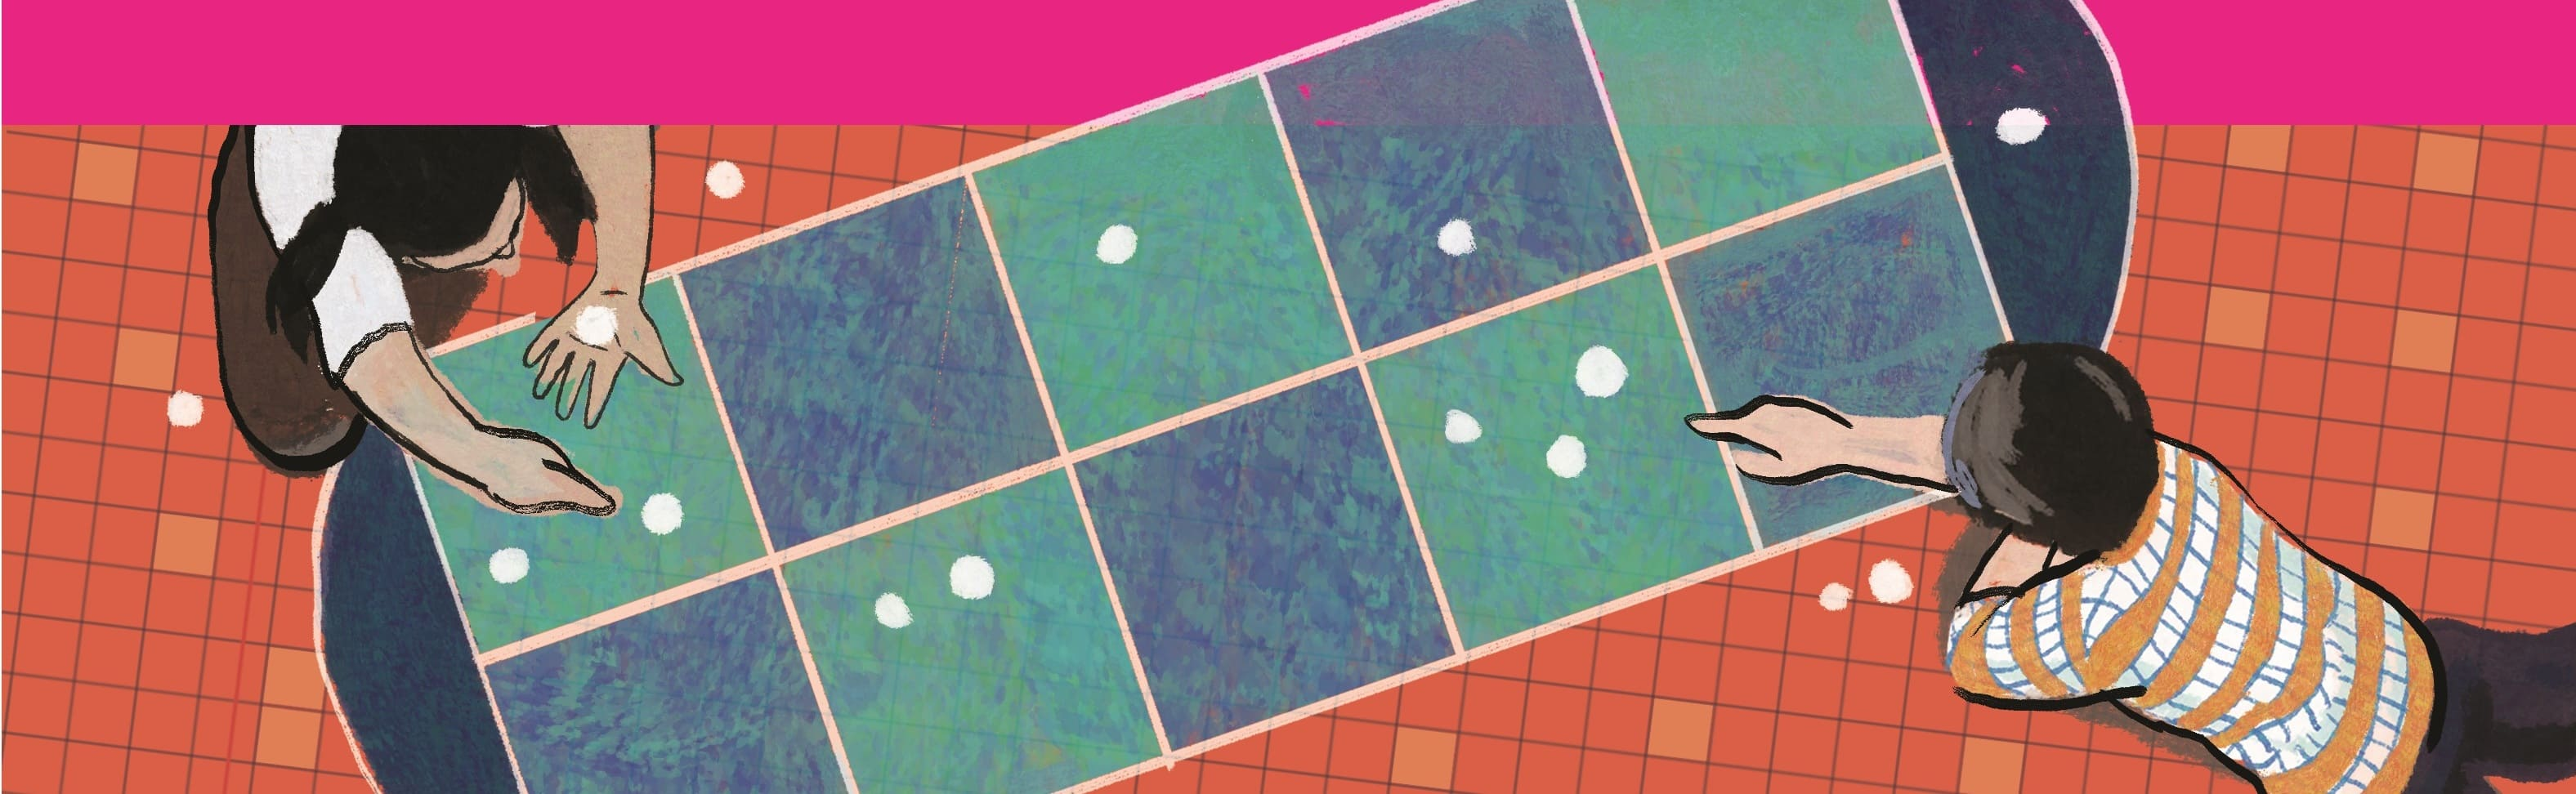
\includegraphics[width=19.3cm]{../bannertoancuabi}}}  
\AddToShipoutPicture*{\put(130,555){
\includegraphics[scale=1]{../tieude.pdf}}} 
\centering
\endgroup
\vspace*{150pt}

\begin{multicols}{2}
	Lần này thì Thám tử Xuân Phong phải vào tận hang ổ của một băng đảng để điều tra manh mối về một vụ án. Khác với những lần bị lạc lên đảo, ở đó có những thổ dân nói thật hoặc nói dối, trong ba người thuộc  băng đảng mà Xuân Phong tiếp cận, không có ai nói thật mà lại có tới ba kiểu người. Loại thứ nhất, tất nhiên rồi, đó là người Nói dối -- chuyên nói sai sự thật. Tiếp theo mới phức tạp cho Xuân Phong, lại có kẻ Ranh mãnh: hắn sẽ nói thật hoặc nói dối bất cứ khi nào hắn muốn. Thế chưa hết, loại cuối cùng mới rầy rà, đó là người Thay đổi, cứ nói thật và nói dối luân phiên nhau. Nhiệm vụ của Thám tử là xác định  từng người thuộc kiểu gì. Vừa được miêu tả về ba kiểu người như vậy, thanh tra Lê Kính đã ôm đầu kêu rên: ``Thôi, thà cho tôi lên hoang đảo với thổ dân nói Thật và nói Dối rõ ràng còn hơn. Ở đây phức tạp tờ mờ quá, không biết đường nào mà lần!"
	\vskip 0.1cm
	Xuân Phong đưa tay trấn an sự bực tức nóng nảy của thanh tra Lê Kính, thì thầm nói: ``Anh cứ yên tâm. Thế giới của băng đảng này phức tạp như vậy, nhưng tôi quả quyết chỉ sau không quá ba câu hỏi, ta sẽ biết ngay ai là thuộc loại người nào?"
	\vskip 0.1cm
	Làm thế nào mà Xuân Phong lại tự tin như thế nhỉ? Em có thể tìm thấy cách Thám tử đặt câu hỏi để xác định ai là ai, và giúp Lê Kính lấy lại bình tĩnh hay không?
\end{multicols}
\begin{figure}[H]
	\centering
	\vspace*{-5pt}
	\captionsetup{labelformat= empty, justification=centering}
	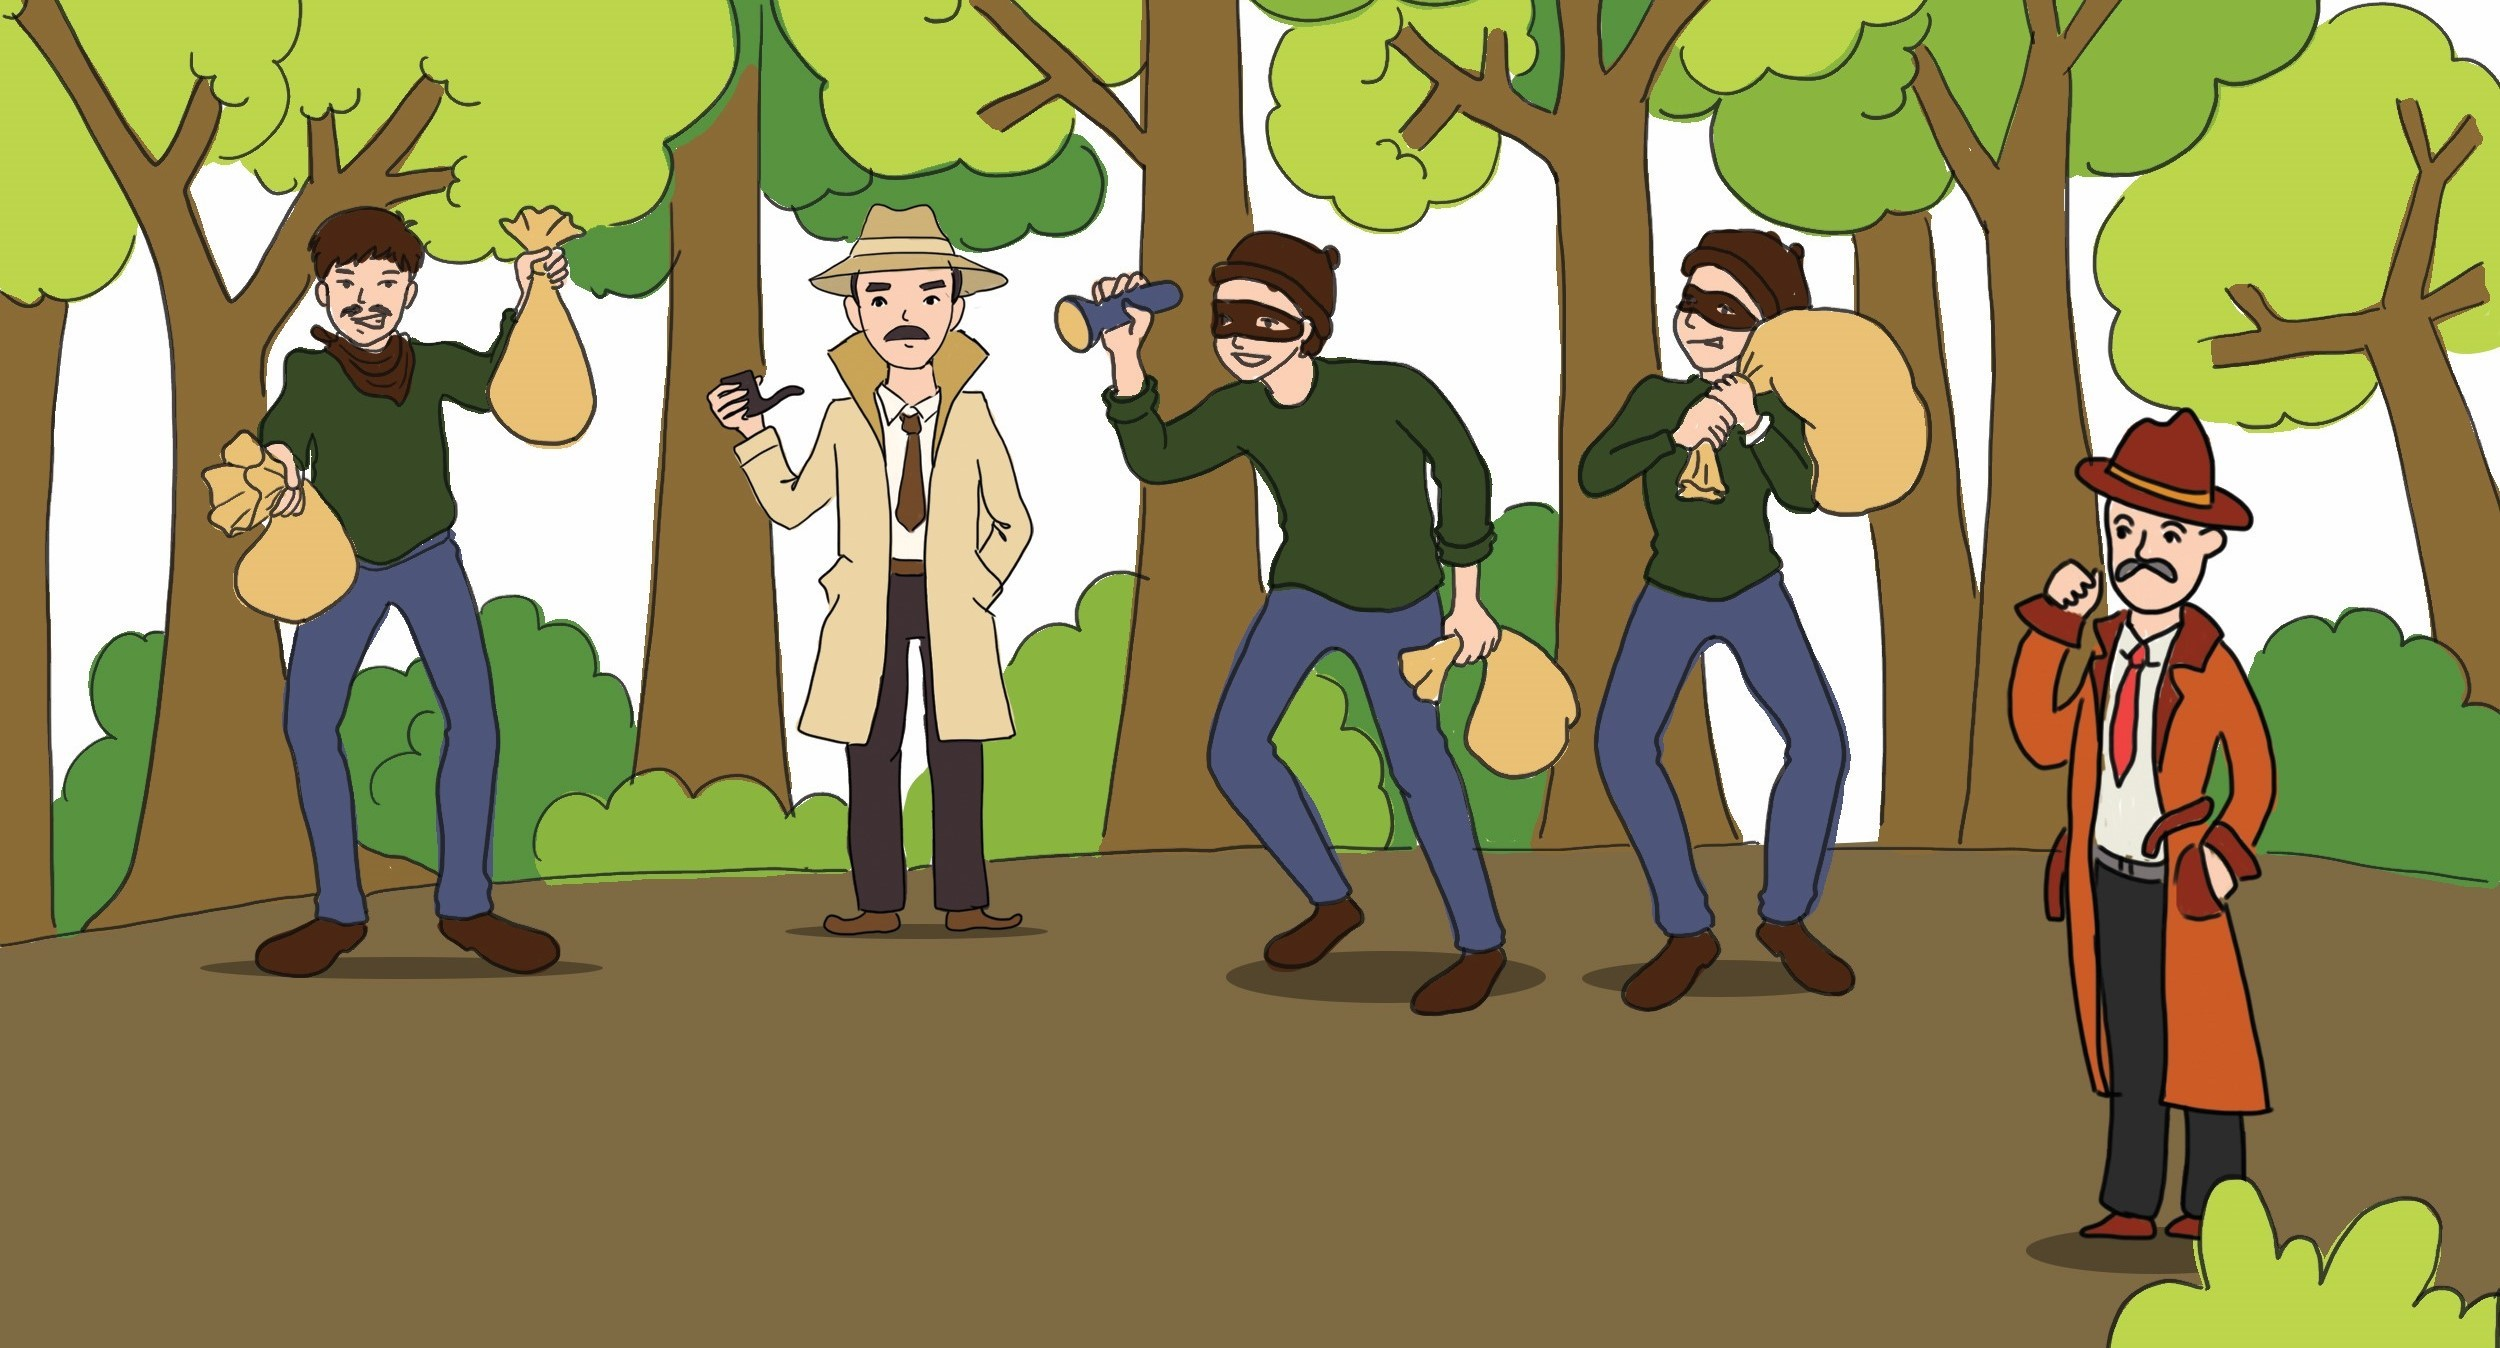
\includegraphics[width=0.98\linewidth]{xuanphong}
	\vspace*{-10pt}
\end{figure}
\newpage
\begingroup
\AddToShipoutPicture*{\put(115,670){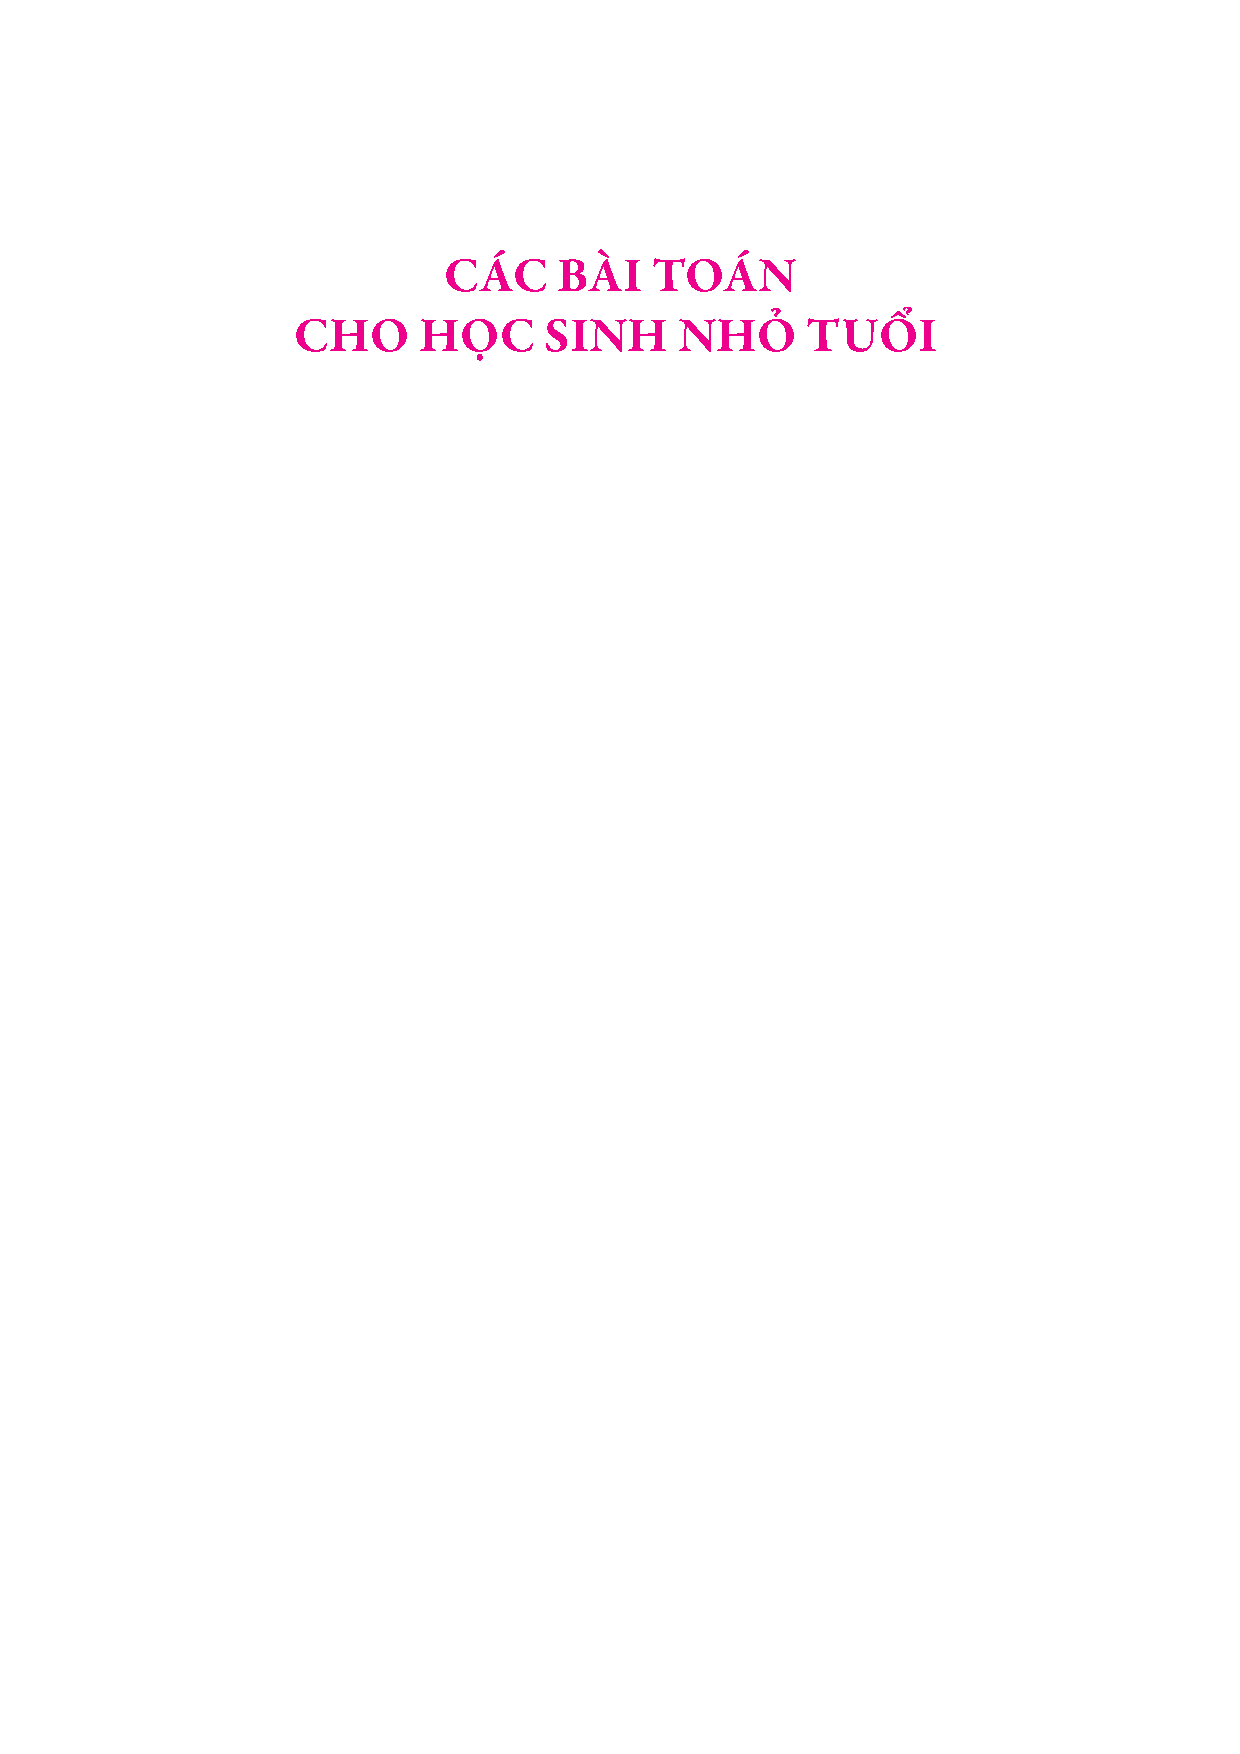
\includegraphics[scale=1]{../tieude11.pdf}}} 
\centering
\endgroup
\vspace*{33pt}

\begin{multicols}{2}
	$\pmb{1.}$	Pinocchio và Pierrot thi chạy với nhau. Pierrot chạy suốt cả quãng đường với cùng một tốc độ, còn Pinocchio chạy nhanh gấp đôi Pierrot trong nửa đầu quãng đường, và nửa sau lại chậm bằng nửa Pierrot. Hỏi ai đã thắng?
	\begin{figure}[H]
		\centering
		\vspace*{-5pt}
		\captionsetup{labelformat= empty, justification=centering}
		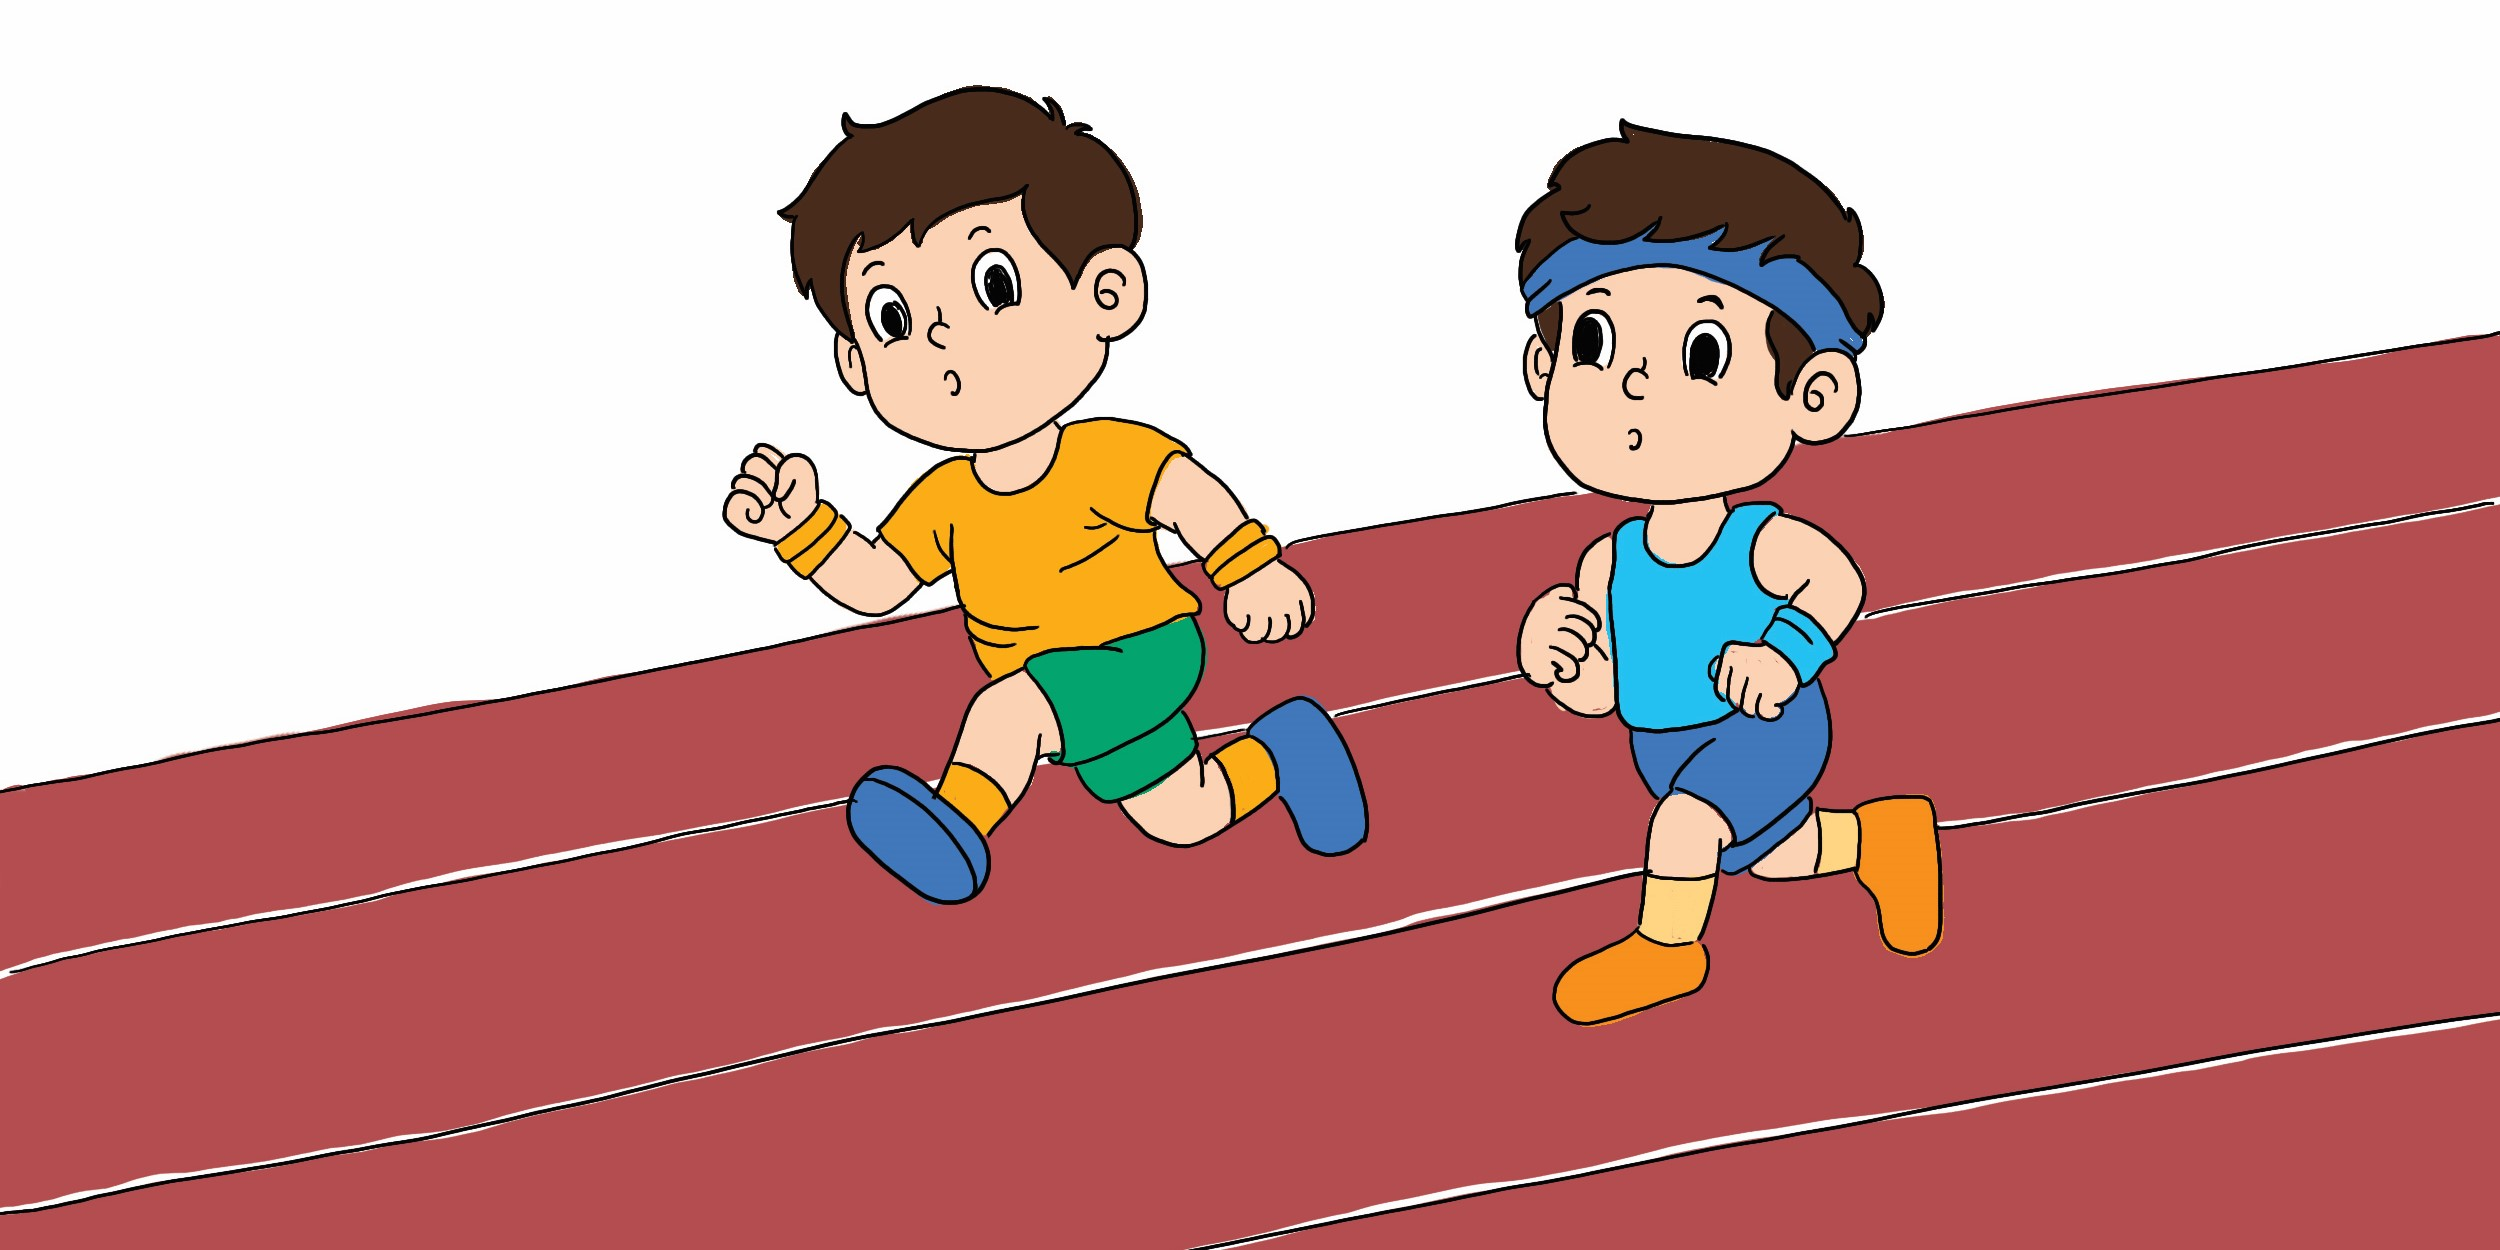
\includegraphics[width=1\linewidth]{Pi4_bai1}
		\vspace*{-15pt}
	\end{figure}
	$\pmb{2.}$ ``Còn quá sớm để các em nhìn thấy điều thần kỳ sau đây của thế giới pháp sư," cô giáo McGonagall  nói với $33$ học trò của mình ở ngôi trường Hogwarts đào tạo Phù thủy, và vung cây đũa thần ra lệnh: ``Nào, các em hãy nhắm mắt lại!" Tất cả học trò nam và một phần ba học trò nữ đều nhắm mắt phải. Tất cả học trò nữ và một phần ba các học trò nam đều nhắm mắt trái. Hỏi có bao nhiêu học trò đã nhìn thấy những gì còn quá sớm để nhìn thấy?
	\begin{figure}[H]
		\centering
		\vspace*{-10pt}
		\captionsetup{labelformat= empty, justification=centering}
		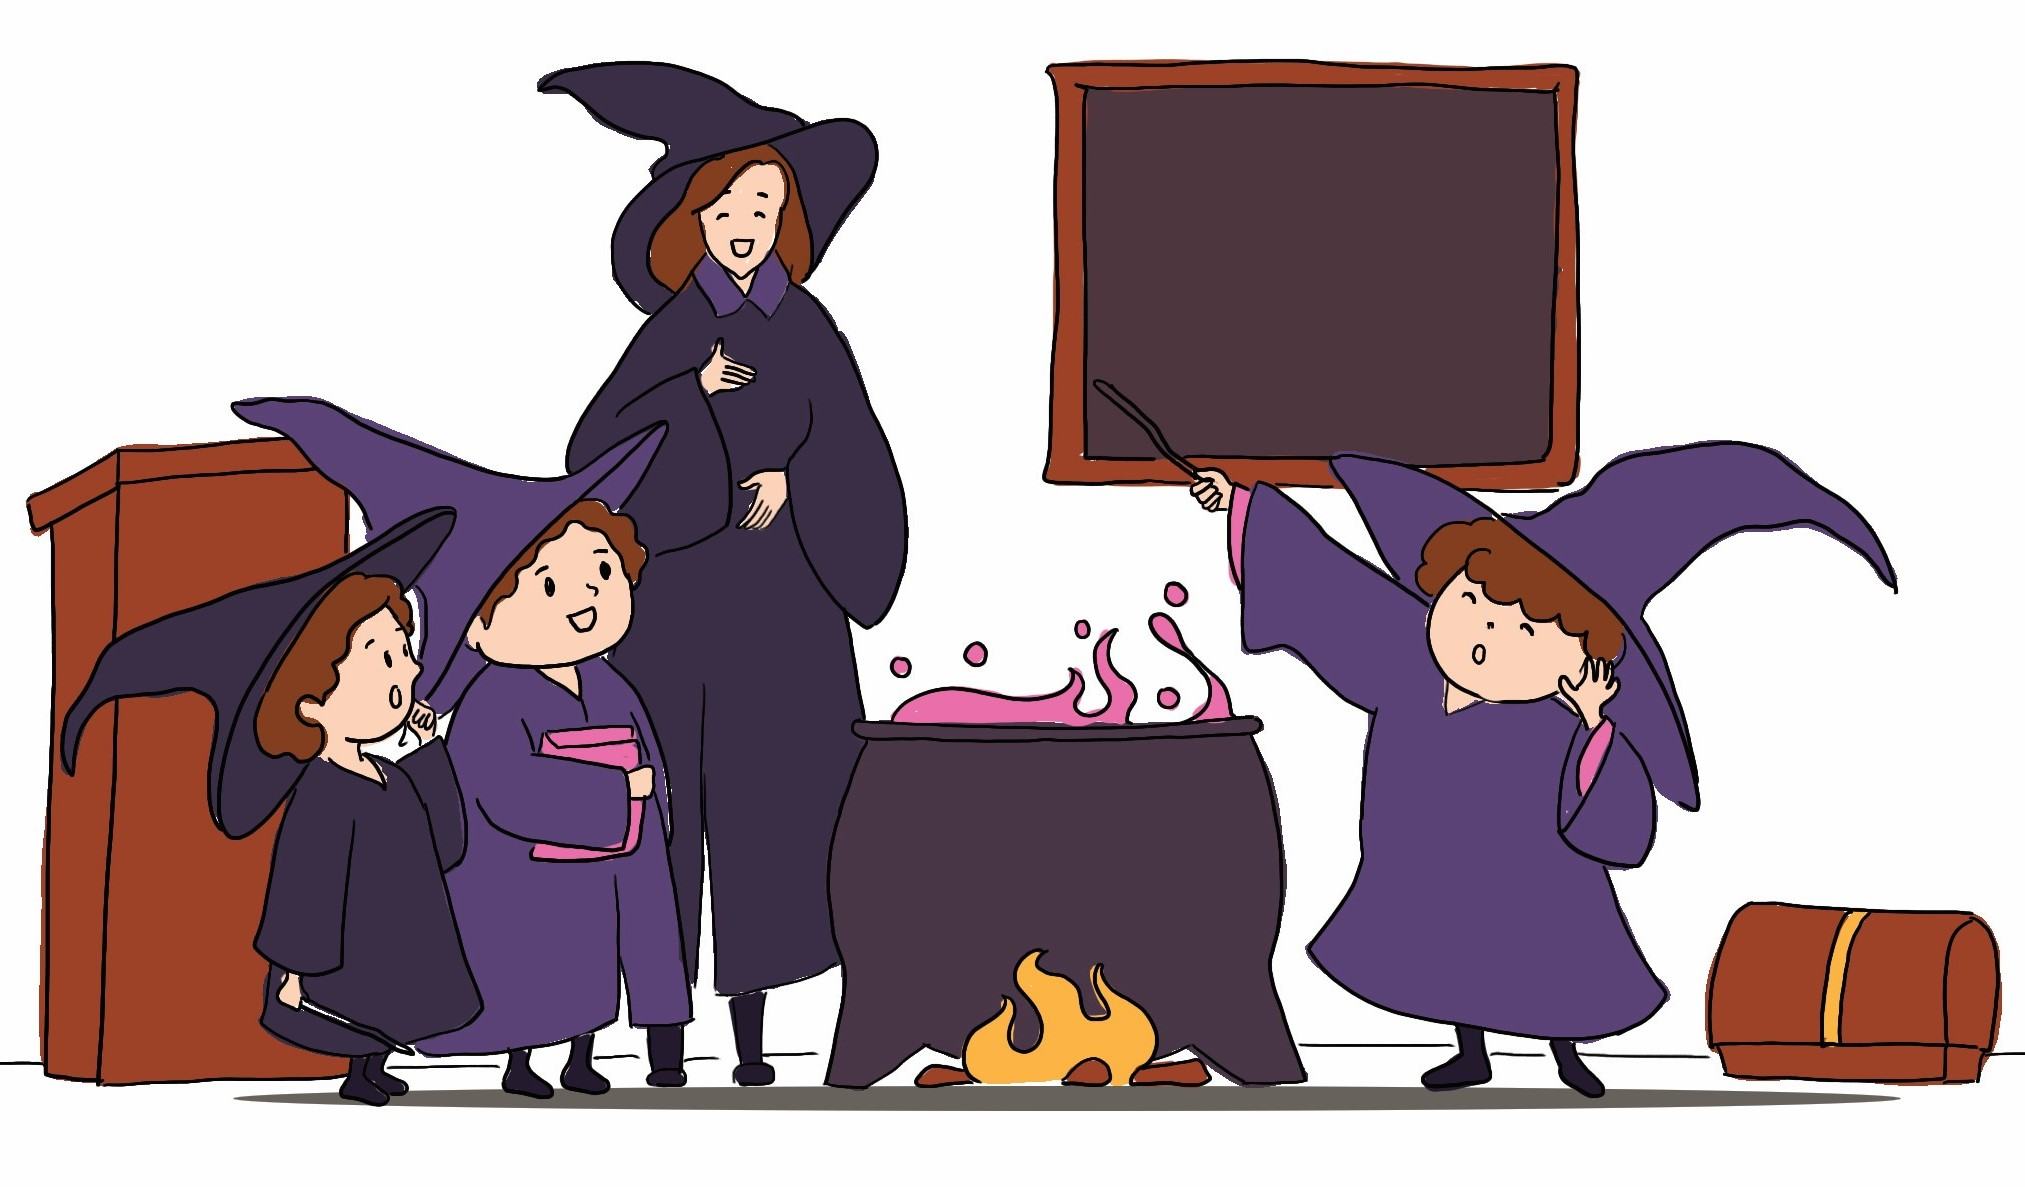
\includegraphics[width=1\linewidth]{Pi4_bai2}
		\vspace*{-15pt}
	\end{figure}
	$\pmb{3.}$ 	Bác Tư múc ra ba thìa sữa từ một ly sữa đầy và đổ chúng vào một ly đựng cà phê nguyên chất và khuấy đều. Sau đó bác múc ba thìa hỗn hợp thu được và đổ lại vào ly sữa. Hỏi bây giờ thứ gì nhiều hơn: cà phê trong ly đựng sữa hay sữa trong ly đựng cà phê?
	\begin{figure}[H]
		\centering
		\vspace*{5pt}
		\captionsetup{labelformat= empty, justification=centering}
		
\includegraphics[width=1\linewidth]{Pi4_bai3}
		\vspace*{-15pt}
	\end{figure}
	$\pmb{4.}$ Ma xó Brownie là một nhân vật trong văn hóa dân gian Anh và một số quốc gia khác. Đó là một dạng Phúc thần (ma thiện), tiểu yêu nghịch ngợm, thường mô tả là bé tí hon, có da nâu, ăn mặc tuềnh toàng, sinh sống gần gũi với con người, và là thần hộ mệnh cho các gia đình. Các Brownies có một xã hội thu nhỏ riêng và thường tổ chức những cuộc họp bí mật tại một tảng đá nào đó để con người không để ý tới. 
	\vskip 0.1cm
	Trong một tòa nhà bảy tầng nọ cũng có rất nhiều ma xó Brownies sinh sống. Thang máy chạy giữa tầng một và tầng cuối, dừng lại ở mỗi tầng. Ở mỗi tầng, bắt đầu từ tầng đầu tiên, có một chú Brownie bước vào thang máy, nhưng không có chú nào bước ra ngoài. Thang máy cứ di chuyển liên tục như vậy cho đến khi chú Brownie thứ một nghìn bước vào thang máy thì thang máy dừng lại. Hỏi điều này đã xảy ra ở tầng nào?
	\begin{figure}[H]
		\centering
		\vspace*{-5pt}
		\captionsetup{labelformat= empty, justification=centering}
		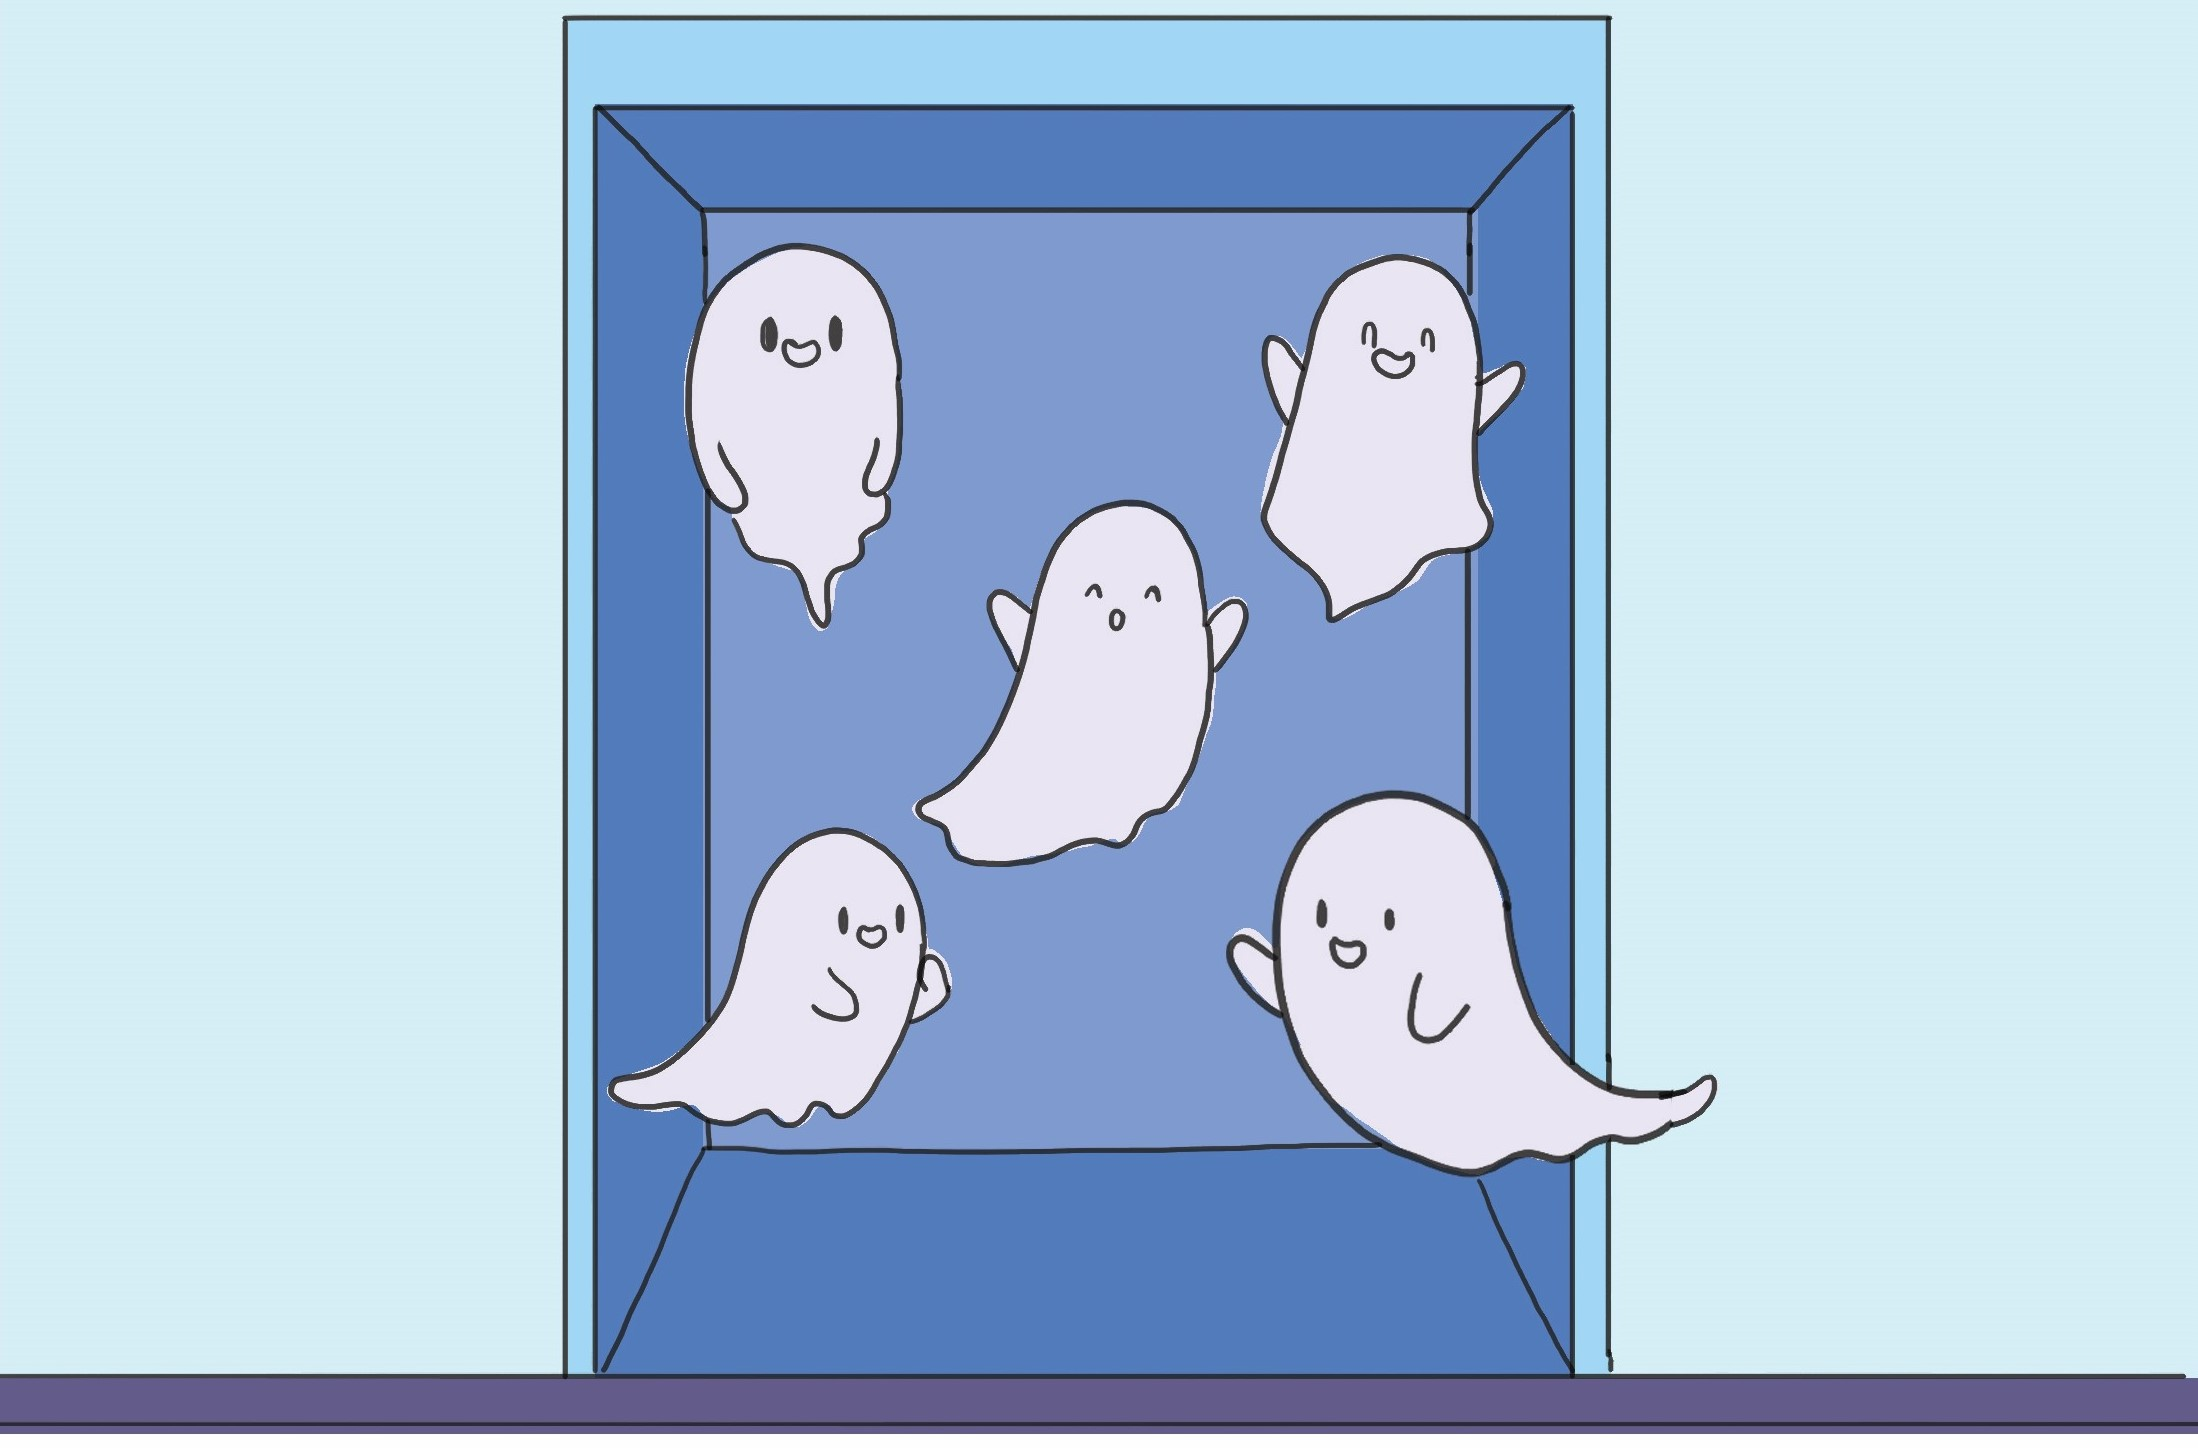
\includegraphics[width=1\linewidth]{Pi4_bai4}
		\vspace*{-20pt}
	\end{figure}
	$\pmb{5.}$ Có $40$ con thú sống trong rừng gồm cáo, sói, thỏ rừng và lửng. Hàng năm, các con thú tổ chức vũ hội hóa trang: mỗi con đeo một chiếc mặt nạ của một loài động vật khác và trong hai năm liên tiếp không con nào đeo cùng một chiếc mặt nạ của cùng một loài.
	\begin{figure}[H]
		\centering
		\vspace*{-5pt}
		\captionsetup{labelformat= empty, justification=centering}
		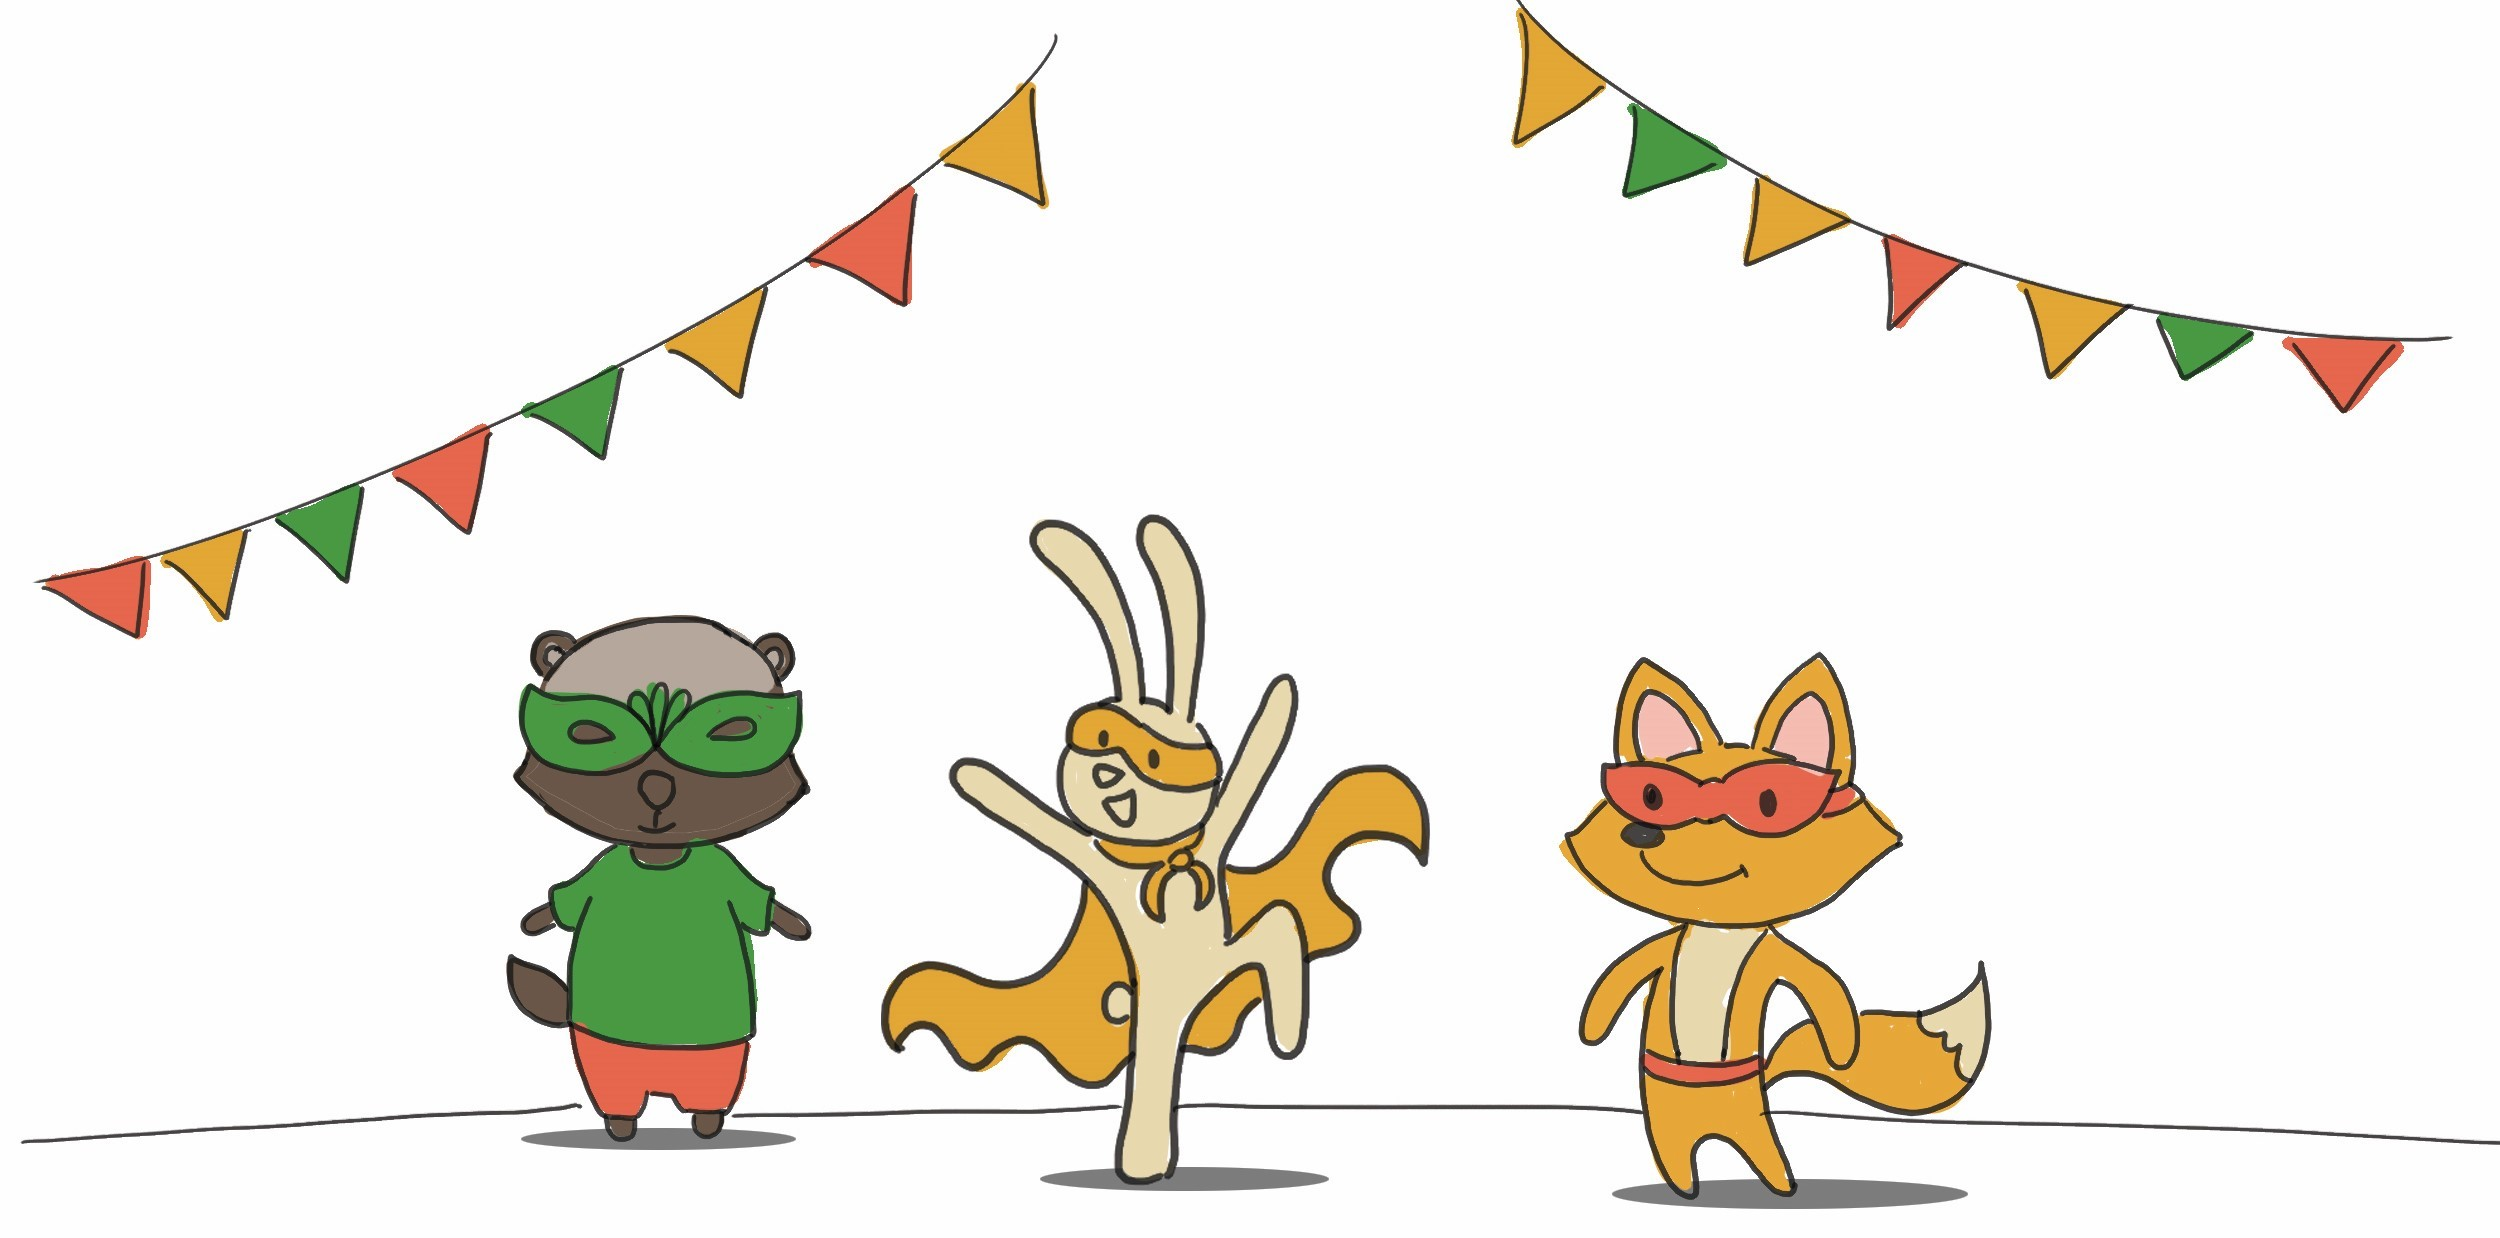
\includegraphics[width=1\linewidth]{Pi4_bai5}
		\vspace*{-20pt}
	\end{figure}
	Hai năm trước, có $12$ ``cáo" và $28$ ``sói" tại vũ hội, một năm trước -- có $15$ ``thỏ rừng", $10$ ``cáo" và $15$ ``lửng", và năm nay -- $15$ ``thỏ rừng" và $25$ ``cáo" . Hỏi loài thú nào có nhiều nhất trong rừng? 
	\vskip 0.1cm
	$\pmb{6.}$ $a)$	Có tám bạn học sinh giải một đề thi gồm $8$ bài toán. Khi tổng kết lại, cô giáo thấy rằng với mỗi bài toán lại có đúng  năm bạn học sinh giải được bài đó. Chứng minh rằng có hai học sinh sao cho với mỗi bài toán trong đề có ít nhất một trong hai em giải được.
	\vskip 0.1cm
	$b)$	Em hãy chỉ ra một ví dụ rằng, nếu với mỗi bài toán đều có đúng bốn bạn học sinh giải được, thì điều khẳng định ở câu $a)$ không đúng.
	\begin{figure}[H]
		\centering
		\vspace*{-10pt}
		\captionsetup{labelformat= empty, justification=centering}
		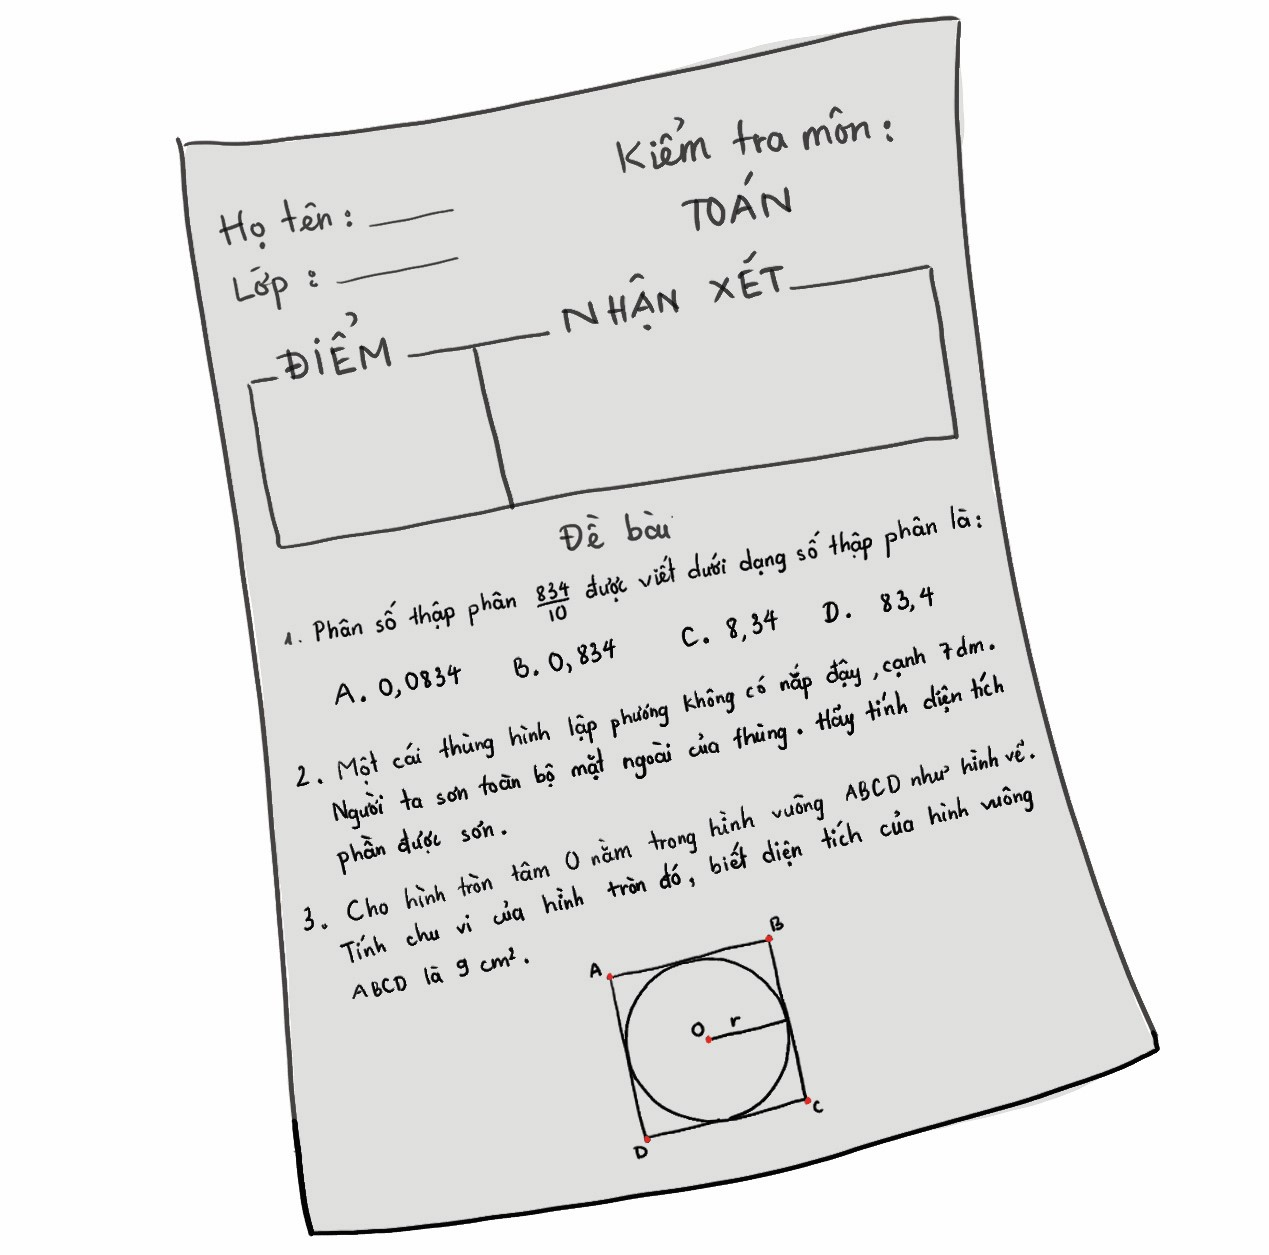
\includegraphics[width=0.7\linewidth]{Pi4_bai6}
		\vspace*{-5pt}
	\end{figure}
\end{multicols}
\vspace*{-10pt}
{\color{toancuabi}\rule{1\linewidth}{0.1pt}}
\begingroup
\AddToShipoutPicture*{\put(110,350){
\includegraphics[scale=1]{../tieude2.pdf}}} 
\centering
\endgroup
\vspace*{75pt}

\begin{multicols}{2}
	$\pmb{1.}$ Bạn Tùng làm một số bài trắc nghiệm và sau đó sẽ lấy điểm trung bình của các bài đó để tự đánh giá học lực của mình. Trả lời xong bài trắc nghiệm cuối cùng, Tùng thấy rằng nếu bài này mình được $97$ điểm thì điểm trung bình của tất cả các bài trắc nghiệm sẽ là $90$ điểm, còn nếu như ở bài cuối Tùng chỉ nhận được $73$ điểm thì điểm trung bình sẽ chỉ còn $87$ điểm. Vậy số bài trắc nghiệm mà Tùng đã làm là bao nhiêu?
	\begin{figure}[H]
		\centering
		\vspace*{-10pt}
		\captionsetup{labelformat= empty, justification=centering}
		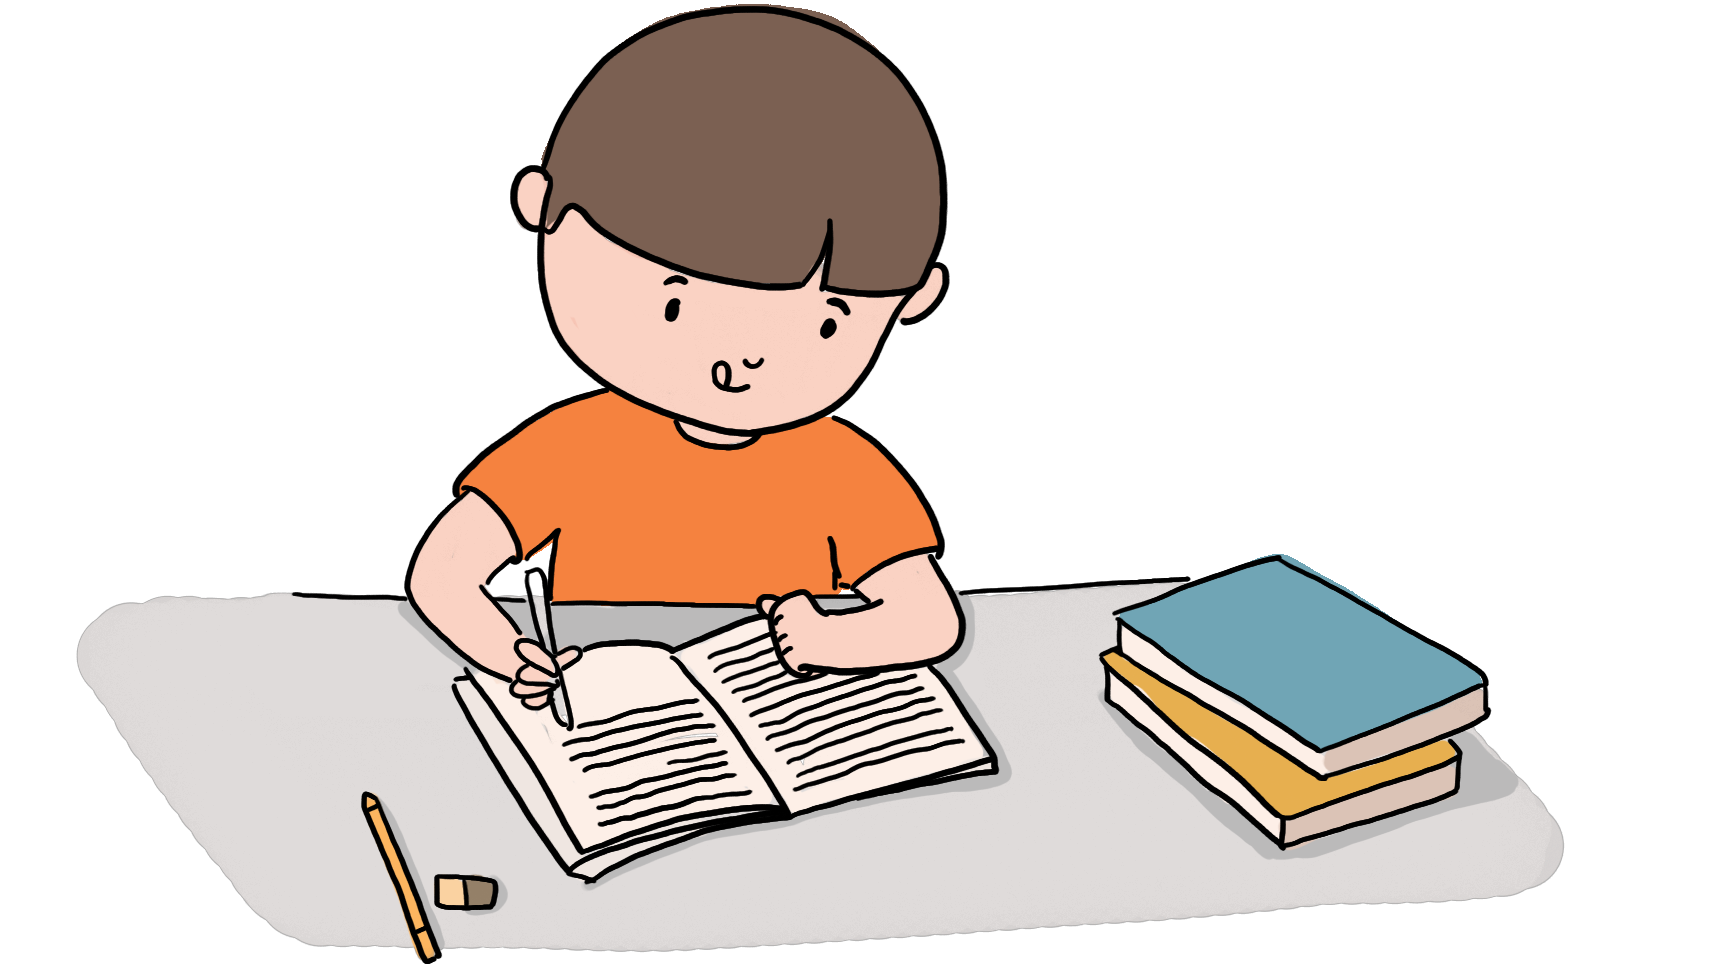
\includegraphics[width=0.98\linewidth]{Pi12_Bai1}
		\vspace*{-5pt}
	\end{figure}
	\textit{Lời giải.} 	Các em có thể gọi số bài trắc nghiệm là $n$, tổng số điểm các bài trắc nghiệm  từ bài số $1$ tới bài thứ $(n-1)$ là $S$. Khi đó ta có các hệ thức sau
	\begin{align*}
		\frac{S + 97}{n} &= 90\\
		\frac{S + 73}{n} &= 87.
	\end{align*}
	Từ đó suy ra $90n-97= 87n-73$. Các em nhận được $n=8$.
	\vskip 0.1cm
	Hoặc các em có thể lập luận nhẩm như sau. Điểm chênh lệch của bài trắc nghiệm  cuối sau hai lần dự tính của Tùng là $97-73 = 24$. Trong khi chênh lệch của hai điểm điểm trung bình là $90-87=3$. Vậy số bài trắc nghiệm  mà Tùng cần thực hiện là \linebreak$\dfrac{24}{3}=8$ (bài).
	\vskip 0.1cm
	$\pmb{2.}$ Có $3$ loại kẹo để trong lọ thủy tinh với ba màu khác nhau: kẹo màu đỏ, kẹo màu vàng và kẹo màu trắng. Nếu Bình nhặt hết số kẹo màu vàng thì tổng số kẹo trong lọ ít hơn một chiếc so với $2/3$ tổng số kẹo ban đầu. Còn nếu Bình nhặt hết số kẹo đỏ, thì số kẹo còn lại trong lọ nhiều hơn $4$ chiếc so với $2/3$ tổng số kẹo ban đầu.
	\vskip 0.1cm
	Vậy ban đầu trong hai loại kẹo màu vàng và kẹo màu trắng, loại nào có nhiều hơn và nhiều hơn bao nhiêu?
	\begin{figure}[H]
		\centering
		\vspace*{-10pt}
		\captionsetup{labelformat= empty, justification=centering}
		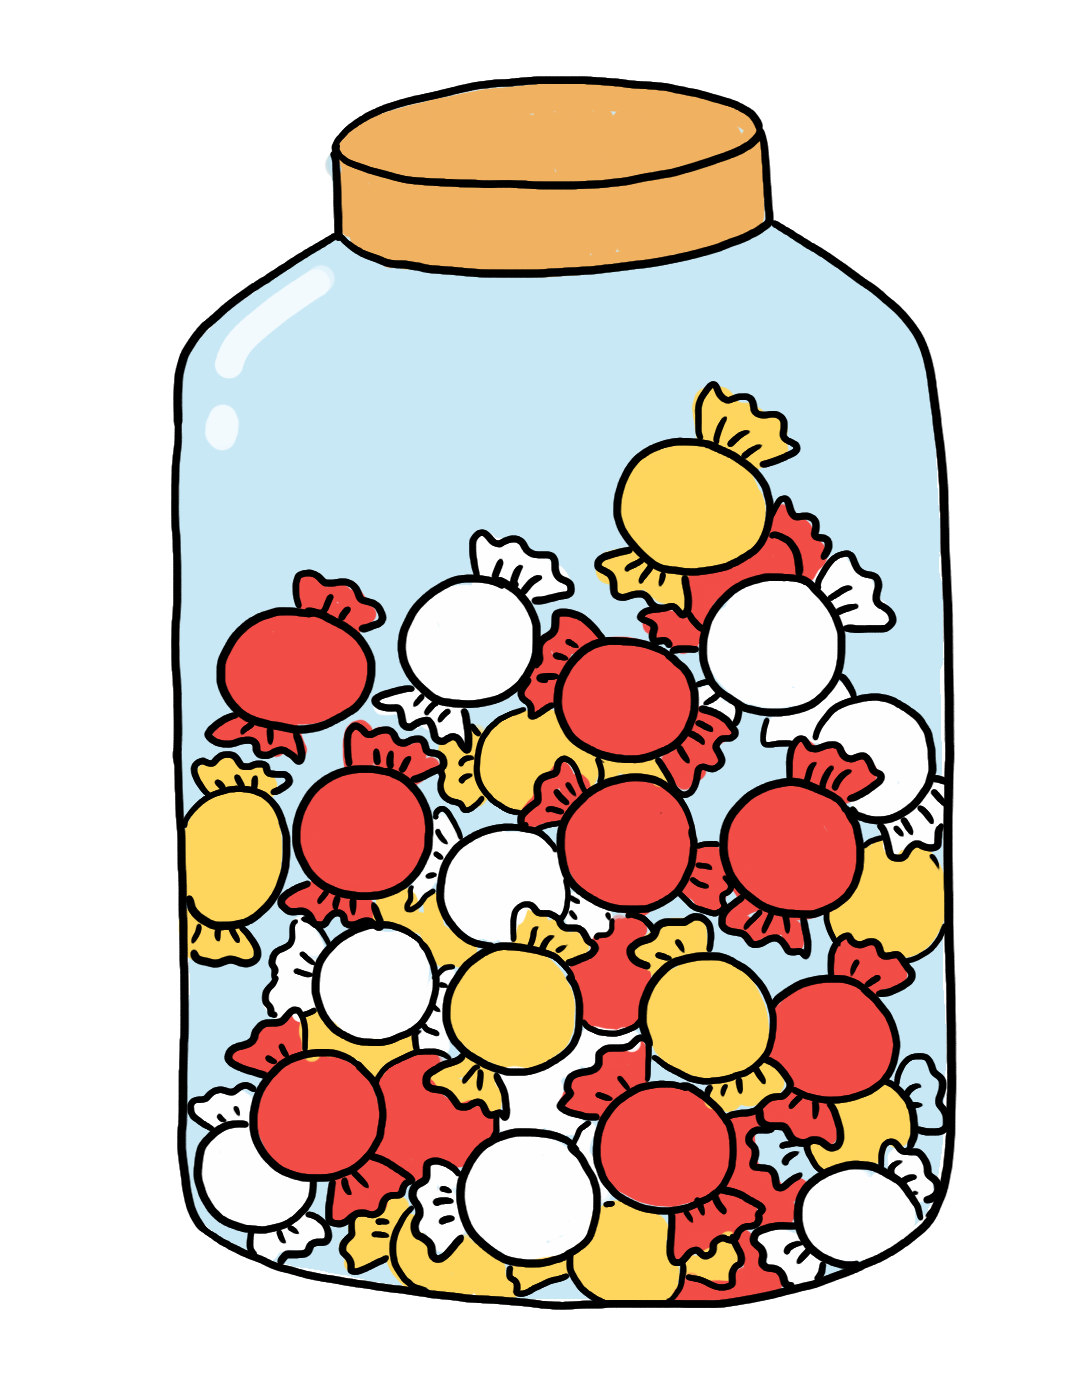
\includegraphics[width=0.45\linewidth]{Pi12_Bai2}
		\vspace*{-15pt}
	\end{figure}
	\textit{Lời giải.} 	Từ điều kiện thứ nhất suy ra số kẹo màu vàng nhiều hơn một chiếc so với $1/3$ tổng số kẹo ban đầu trong lọ. Từ điều kiện thứ hai suy ra số kẹo màu đỏ ít hơn $4$ chiếc so với $1/3$ tổng số kẹo ban đầu trong lọ. Suy ra số kẹo màu trắng  nhiều hơn $(4-1)=3$ chiếc so với $1/3$ tổng số kẹo ban đầu, tức là nhiều hơn $2$ chiếc so với số kẹo màu vàng.
	\vskip 0.1cm
	$\pmb{3.}$ $40$ bạn nhỏ nắm tay nhau xếp thành vòng tròn quanh đống lửa trại. Có tất cả $22$ bạn có nắm tay một bạn nam, và $30$ bạn có nắm tay một bạn nữ. Hỏi có tất cả bao nhiêu bạn nữ xếp trong vòng tròn quanh lửa trại ngày hôm đó?
	\begin{figure}[H]
		\centering
		\vspace*{-10pt}
		\captionsetup{labelformat= empty, justification=centering}
		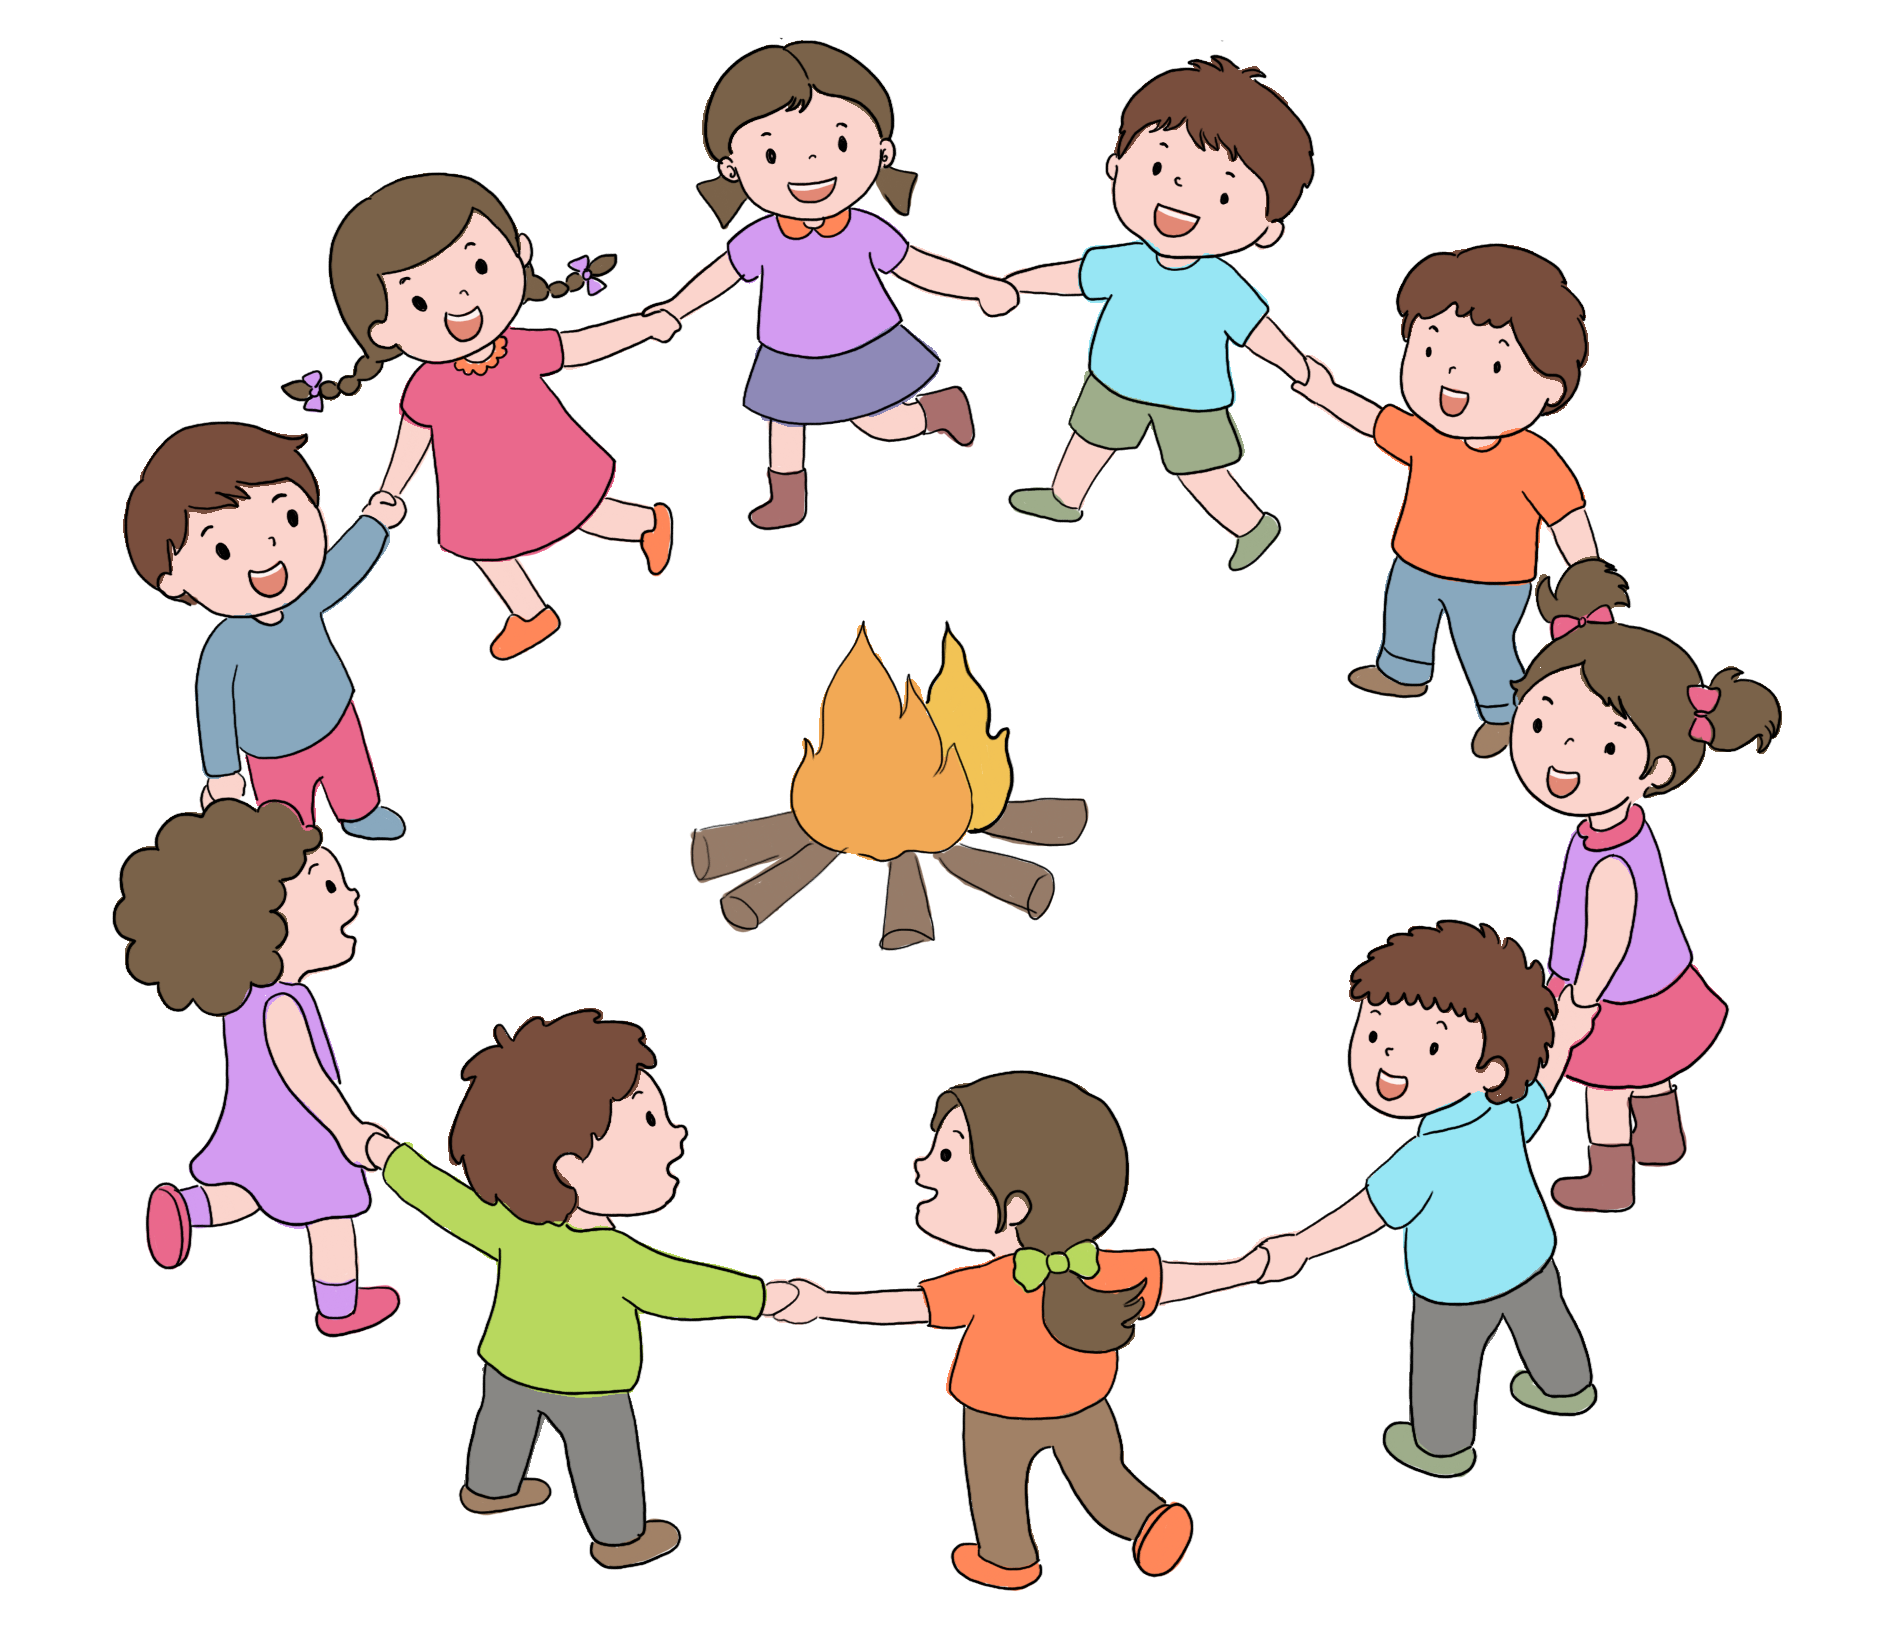
\includegraphics[width=0.9\linewidth]{Pi12_Bai3}
		\vspace*{-5pt}
	\end{figure}
	\textit{Lời giải.} 	Vì $22+30=52$ và $52-40 = 12$, nên có $12$ bạn nhỏ hôm đó vừa nắm tay cả bạn nam lẫn bạn nữ trong vòng tròn. Suy ra có $30-12=18$ bạn chỉ nắm tay các bạn nữ.  $18$ bạn này nắm tất cả $18\times2=36$ cánh tay của các bạn nữ, còn $12$ bạn còn lại nắm đúng $12$ cánh tay của các bạn nữ. Vì thế tổng số cánh tay của các bạn nữ là $36+12=48$. Do đó số các bạn nữ là $48:2=24$ (bạn).
	\vskip 0.1cm
	$\pmb{4.}$ Trên mặt bàn có $5$ đồng xu xếp thành hàng ngang. Đồng xu ở giữa đặt sấp còn $4$ đồng còn lại đều đặt ngửa. Mỗi một lần em được phép lật $3$ đồng xu đặt liền nhau tùy ý. Liệu em có thể có cách lật thế nào để cuối cùng $5$ đồng xu đều đặt sấp được không?
	\vskip 0.1cm
	Cũng câu hỏi như vậy, nếu lúc đầu đồng xu đặt sấp duy nhất là đồng xu xếp đầu hàng? Là đồng xu xếp thứ hai trong hàng?
	\begin{figure}[H]
		\centering
		\vspace*{-5pt}
		\captionsetup{labelformat= empty, justification=centering}
		
\includegraphics[width=1\linewidth]{Pi12_Bai4}
		\vspace*{-20pt}
	\end{figure}
	\textit{Lời giải.} Nếu lúc đầu đồng ở giữa là đồng duy nhất đặt xấp, thì em chỉ cần lật $3$ đồng xu xếp đầu tiên, sau đó lại lật $3$ đồng xu xếp cuối hàng là hoàn thành nhiệm vụ.
	\vskip 0.1cm
	Nếu lúc đầu đồng xu thứ hai là đồng đặt xấp duy nhất, thì em không thể nào lật xấp toàn bộ $5$ đồng xu. Thật vậy, có ba cách lật ba đồng xu đặt cạnh nhau: lật $3$ đồng xu đầu tiên, $3$ đồng xu ở giữa và $3$ đồng xu cuối hàng ngang. Do lúc đầu đồng xu đầu hàng và đồng xu cuối hàng đều đặt ngửa, nên mỗi một trong số hai đồng xu này phải lật một số lẻ lần, có nghĩa là hai cách “lật” kiểu thứ nhất và kiểu thứ ba phải thực hiện một số lẻ lần. Khi đó, với hai kiểu “lật” này đồng xu ở giữa sẽ bị lật một số chẵn lần (do \textit{lẻ $+$ lẻ $=$ chẵn}). Nhưng lúc đầu đồng xu ở giữa đặt ngửa nên số lần “lật” kiểu thứ hai cũng phải là số lẻ. Tuy nhiên, khi đó đồng xu thứ tư lại sẽ bị lật một số chẵn (\textit{$=$ lẻ $+$ lẻ}) lần, và nó cuối cùng sẽ vẫn bị lật ngửa. Do đó, trong trường hợp này em không thể lật xấp tất cả các đồng xu.
	\vskip 0.1cm
	Lý luận tương tự, em cũng có thể thấy không thể lật xấp cả $5$ đồng xu nếu lúc đầu đồng xu đứng đầu hàng là đồng xu duy nhất  được đặt xấp.
	\vskip 0.1cm
	$\pmb{5.}$ Một lần Lý Toét diện guốc mộc loẹt quẹt ra tận chợ phiên chơi ngày cuối tuần. Khi về nhà, Lý Toét ba hoa khoe khắp làng ``Tôi là tôi gặp $15$ ông bán cây cảnh ngoài chợ nhé. Mà tôi đi lòng vòng và nghiệm thấy cứ $3$ ông bất kỳ có tổng cộng đúng $10$ cây hoa hồng. Thế là tôi lẩm nhẩm đoán được ngay $15$ ông này có tất cả bao nhiêu cây hoa hồng."
	\vskip 0.1cm
	Em có thể đoán được Lý Toét đã tính số cây hoa hồng của $15$ ông bán cây cảnh như thế nào không? Hay Lý Toét có khoác lác hay nhầm lẫn gì không nhỉ?
	\begin{figure}[H]
		\centering
		\vspace*{-5pt}
		\captionsetup{labelformat= empty, justification=centering}
		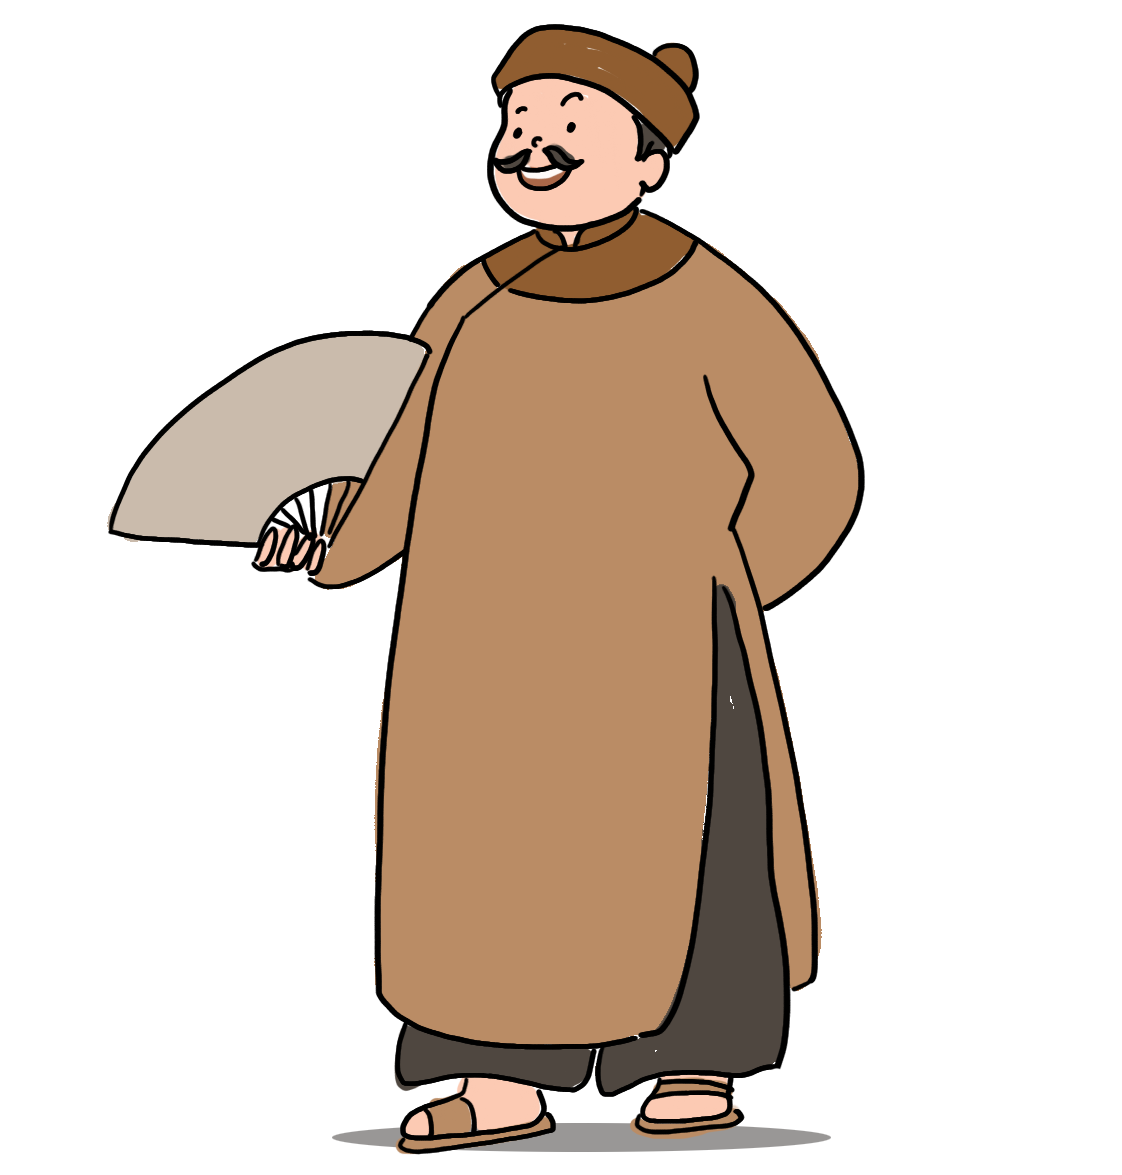
\includegraphics[width=0.58\linewidth]{Pi12_Bai5}
		\vspace*{-10pt}
	\end{figure}
	\textit{Lời giải.} Trước tiên ta sẽ chỉ ra hai ông bán cây bất kỳ luôn có số cây hồng bằng nhau. Gọi hai ông đó là $A$ và $B$. Lấy thêm hai ông $C$ và $D$ khác nữa trong số $15$ ông bán cây. Theo lời của Lý Toét, $3$ ông $A$, $C$ và $D$ có $10$ cây hồng. Và cũng thế, $3$ ông $B$, $C$, $D$ cũng có đúng $10$ cây hồng. Suy ra  ông $A$ và ông $B$ có số cây hồng bằng nhau.  Vì hai ông này được chọn bất kỳ, suy ra số cây hồng của mỗi ông trong số $15$ ông là như nhau.
	\vskip 0.1cm
	Nhưng khi đó, ba ông bán cây không thể có đúng $10$ cây hồng vì số cây phải là số nguyên, mà $10$ lại không chia hết cho $3$.
	\vskip 0.1cm
	Vì thế, chắc chắn Lý Toét có hơi khoác lác hoặc nhầm lẫn đấy. 
	\vskip 0.1cm
	$\pmb{6.}$ Có $20$ bạn tham gia nhóm Toán ngồi xung quanh một chiếc bàn tròn. Một lúc sau các bạn nhóm Văn cũng đến, cứ xen kẽ hai bạn nhóm Toán ngồi kề nhau giờ có thêm $20$ bạn mới từ nhóm Văn. Tổng cộng có tất cả $400$ bạn từ nhóm Văn ngồi thêm quanh chiếc bàn tròn rộng đó. Thỉnh thoảng một bạn nhóm Văn lại đứng dậy và rời khỏi bàn, dắt theo hai bạn ngồi cạnh mình đi luôn. Cứ như vậy, sau một lúc thì quanh bàn số bạn nhóm Toán còn lại chỉ là $3$ bạn. Hỏi số bạn nhóm Văn còn ở lại quanh bàn lúc đó ít nhất phải là bao nhiêu?
	\vskip 0.1cm
	\textit{Lời giải.} 	Các bạn nhóm Toán chia chiếc bàn tròn ra thành các khoảng bao gồm các bạn nhóm Văn ngồi giữa. Ta sẽ chỉ ra một tính chất (bất biến!) thú vị quan trọng sau: trong mỗi khoảng như vậy số các bạn nhóm Văn luôn là một số chia $3$ dư $2$. Thật vậy, điều này lúc đầu là đúng vì $20$ chia $3$ dư $2$. Nếu có $3$ bạn nhóm Văn rời khỏi bàn thì số bạn nhóm Văn trong một khoảng nào đó sẽ giảm đi $3$. Nếu có $1$ bạn nhóm Toán và $2$ bạn nhóm Văn rời khỏi bàn, thì hai khoảng sẽ nhập lại thành $1$ và tổng số bạn nhóm Văn trong khoảng tổng cộng mới đó sẽ giảm đi $2$.  Trong khoảng mới này, số bạn nhóm Văn sẽ chia $3$ dư $(2+2)-2 = 2$, có nghĩa là tính chất vẫn giữ nguyên. Cũng theo lập luận này, không thể xảy ra tình huống có $1$ bạn nhóm Văn rời bàn mang theo hai bạn nhóm Toán, vì khi đó trong khoảng giữa hai bạn nhóm Toán chỉ có $1$ bạn Văn, mà $1$ chia $3$ không thể dư $2$.
	\vskip 0.1cm
	Suy ra tính chất đó sẽ vẫn đúng ở thời điểm cuối cùng. Khi đó có $3$ bạn nhóm Toán ngồi lại, chia bàn ra $3$ khoảng, và trong mỗi khoảng phải có ít nhất $2$ bạn nhóm Văn. Suy ra số bạn nhóm Văn còn lại ngồi quanh bàn là $6$ bạn. 
	\vskip 0.1cm
	Ta có thể xây dựng tình huống để quanh bàn còn ngồi lại đúng $6$ bạn nhóm Văn như sau. Đầu tiên, $17$ bạn nhóm Toán rời khỏi bàn lần lượt, chỉ để lại $3$ bạn nhóm Toán ở lại. Sau đó mỗi một khoảng gồm các bạn nhóm Văn sẽ giảm dần cho đến khi chỉ còn $2$ bạn nhóm Văn ở lại khoảng đó.
\end{multicols}
\newpage
\begingroup
\thispagestyle{toancuabinone}
\blfootnote{$^1$\color{toancuabi}Ottawa, Canada.}
\AddToShipoutPicture*{\put(60,733){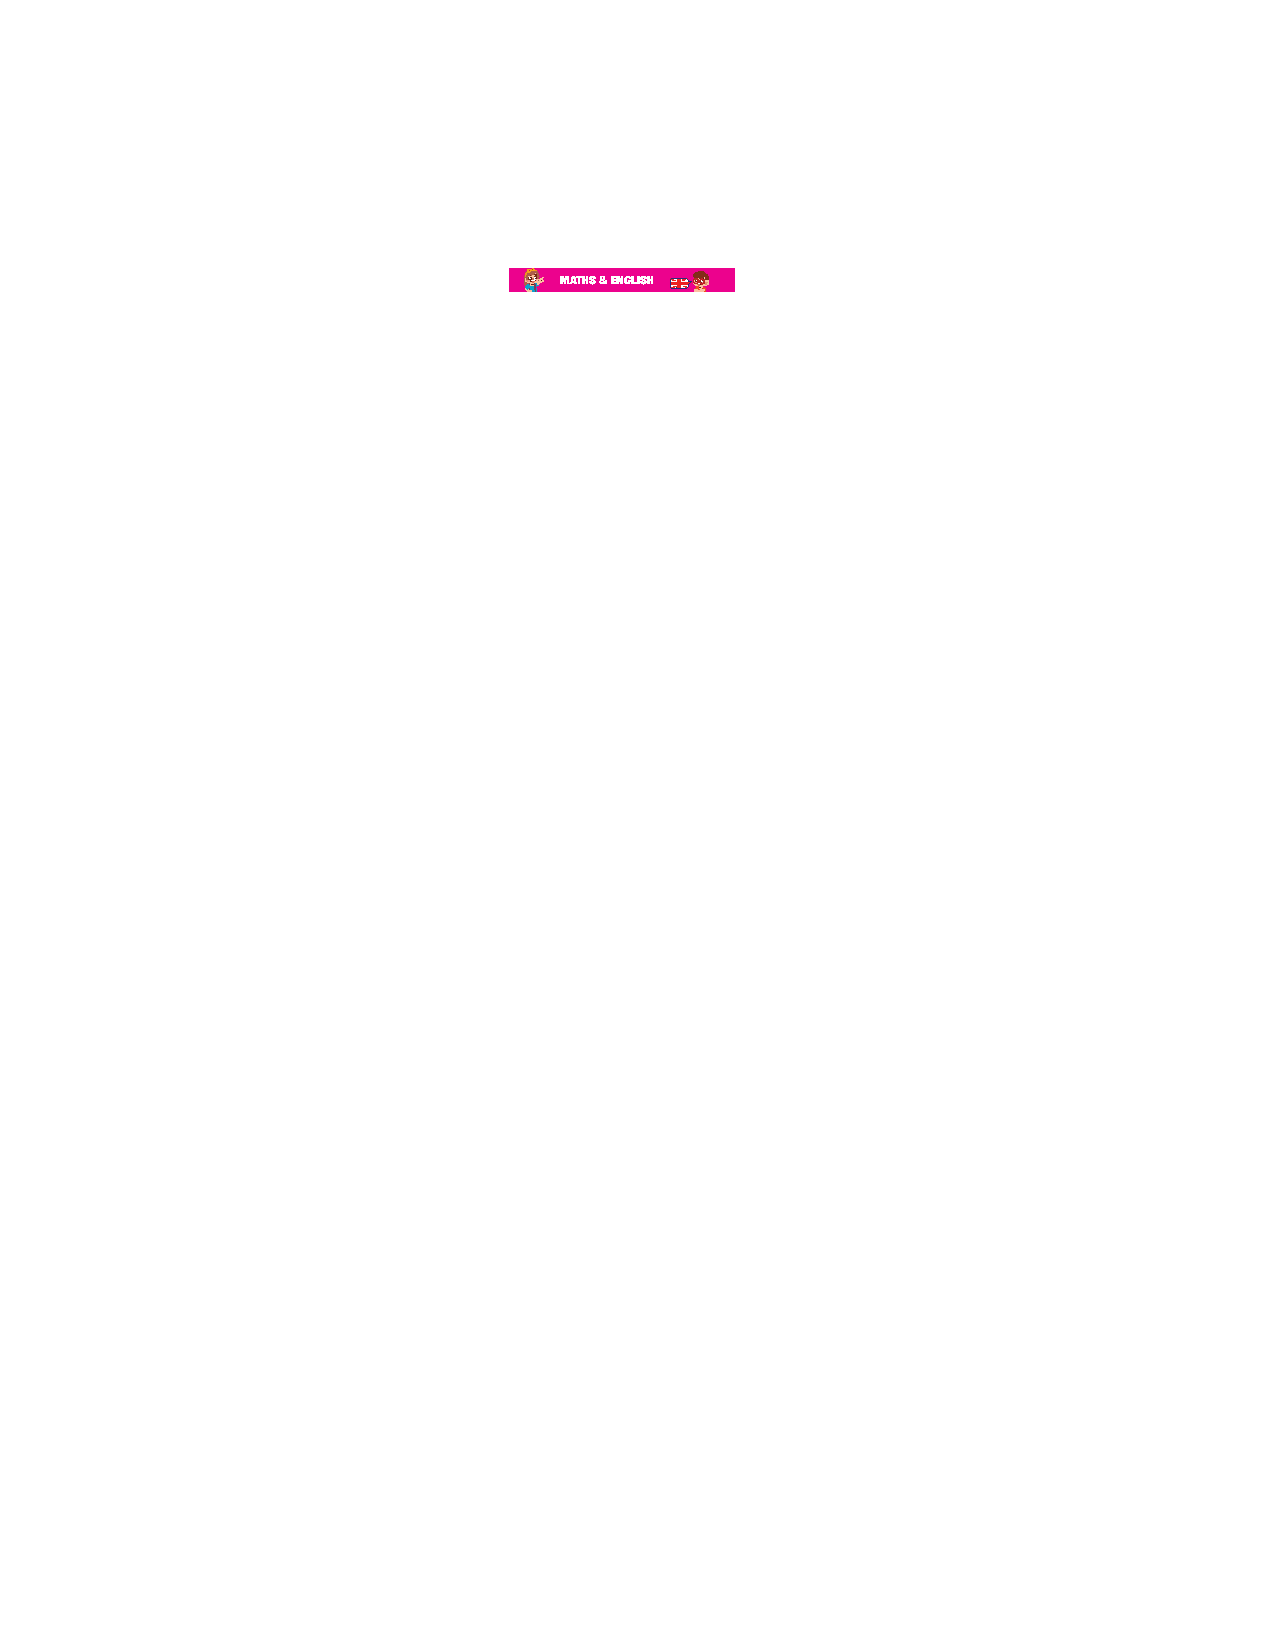
\includegraphics[width=17.2cm]{../mathc.pdf}}}
%\AddToShipoutPicture*{\put(-2,733){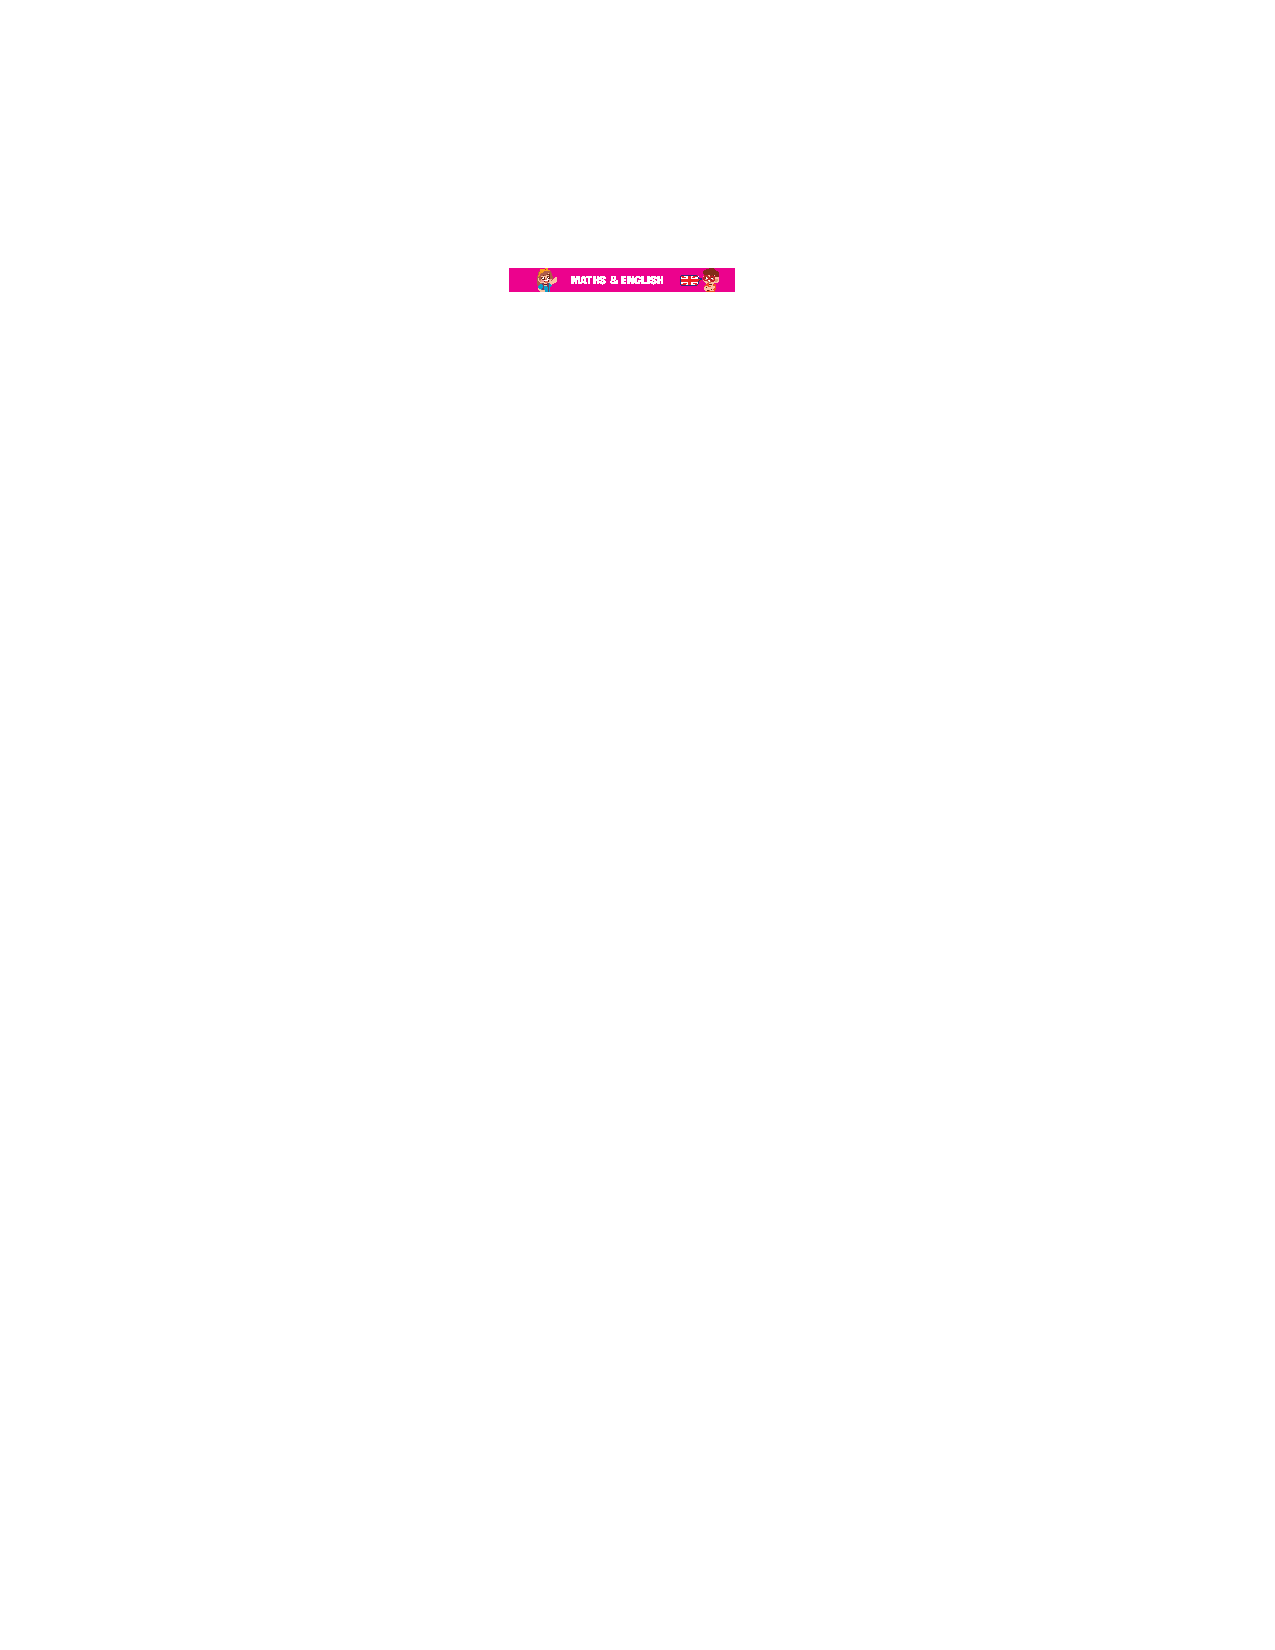
\includegraphics[width=17.2cm]{../mathl.pdf}}} 
\AddToShipoutPicture*{\put(145,680){
\includegraphics[scale=1]{../tieude3.pdf}}} 
\centering
\endgroup
\vspace*{25pt}

\begin{multicols}{2}
	In this article, we introduce an application of graph theory to pattern recognition.
	\vskip 0.2cm
	\PIbox{
		{\color{toancuabi}\textbf{Exercise} (Phrase matching)\textbf{.}} Match the Vietnamese phrases in the left column to their English translations in the right column of the table below.}
	\begin{table}[H]
		\vspace*{-5pt}
		\centering
		\captionsetup{labelformat= empty, justification=centering}
		\renewcommand{\arraystretch}{1.2}
		\setlength{\tabcolsep}{4pt}
		\resizebox{\columnwidth}{!}{\begin{tabular}{|c|l|c|c|l|}
				\cline{1-2} \cline{4-5}
				\multirow{ 2}{*}{$1$}  & \multirow{ 2}{*}{băng}       &  & \multirow{ 2}{*}{A} & bouquet (a bunch        \\
				&      &  & &of flowers)        \\
				\cline{1-2} \cline{4-5} 
				$2$  & bó         &  & B & chalk                               \\ \cline{1-2} \cline{4-5} 
				$3$  & bó hoa     &  & C & circle                              \\ \cline{1-2} \cline{4-5} 
				$4$  & cánh hoa   &  & D & cluster                              \\ \cline{1-2} \cline{4-5} 
				$5$  & đá         &  & E & detour                              \\ \cline{1-2} \cline{4-5} 
				$6$  & đá lửa     &  & F & fire                                \\ \cline{1-2} \cline{4-5} 
				\multirow{ 2}{*}{$7$}  & \multirow{ 2}{*}{đá phấn}    &  & \multirow{ 2}{*}{G} & flint (a stone used \\
				&     &  &  & to make sparks) \\
				\cline{1-2} \cline{4-5} 
				$8$  & đường      &  & H & flower                              \\ \cline{1-2} \cline{4-5} 
				$9$  & đường vòng &  & I & ice                                 \\ \cline{1-2} \cline{4-5} 
				$10$ & hoa        &  & J & iceberg                             \\ \cline{1-2} \cline{4-5} 
				$11$ & lửa        &  & K & mountain                            \\ \cline{1-2} \cline{4-5} 
				$12$ & mở         &  & L & petal                               \\ \cline{1-2} \cline{4-5} 
				$13$ & mở đường   &  & M & pollen                              \\ \cline{1-2} \cline{4-5} 
				$14$ & mở mắt     &  & N & powder                              \\ \cline{1-2} \cline{4-5} 
				$15$ & núi        &  & O & road                                \\ \cline{1-2} \cline{4-5} 
				$16$ & núi băng   &  & P & rock                                \\ \cline{1-2} \cline{4-5} 
				$17$ & núi lửa    &  & Q & tear (as in teardrop)               \\ \cline{1-2} \cline{4-5} 
				$18$ & nước đá    &  & R & to make aware                       \\ \cline{1-2} \cline{4-5} 
				$19$ & nước mắt   &  & S & to open                             \\ \cline{1-2} \cline{4-5} 
				$20$ & phấn       &  & T & to pave the way                     \\ \cline{1-2} \cline{4-5} 
				$21$ & phấn hoa   &  & U & volcano                             \\ \cline{1-2} \cline{4-5} 
				$22$ & vòng       &  & V & wreath                              \\ \cline{1-2} \cline{4-5} 
				$23$ & vòng hoa   &  &   &                                     \\ \cline{1-2} \cline{4-5} 
		\end{tabular}}
		\vspace*{-10pt}
	\end{table}
\textit{Solution.}
We use a graph theory approach from the point of view of an English speaker to solve the problem.
\vskip 0.1cm
First, notice that the Vietnamese phrases above are single--word and double--word phrases.
We construct a graph as follows: each phrase is represented by a vertex; an edge connects a single--word phrase and a double--word phrase where the latter contains the former.  See the graph below.
\begin{figure}[H]
	\vspace*{-5pt}
	\centering
	\captionsetup{labelformat= empty, justification=centering}
	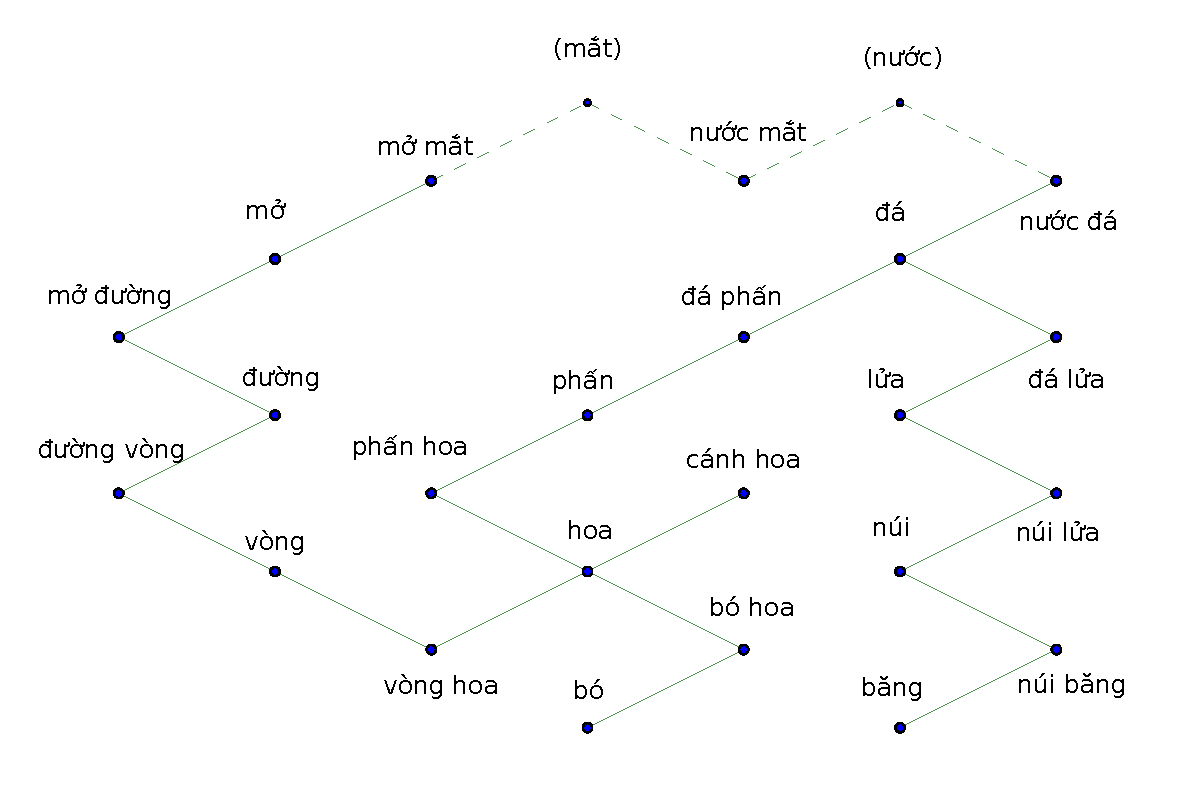
\includegraphics[width= 1\linewidth]{hc-2022-2-2-2-1.pdf}
	\caption{\small\textit{\color{toancuabi}Graph of Vietnamese phrases}}
	\vspace*{-10pt}
\end{figure}
In plain words, the graph of Vietnamese phrases represents connections in \textit{shared meaning} between the connected phrases.
Similarly, we connect the English phrases such that, in each connected phrases, the meaning of one phrase is contained in the meaning of the other.
We obtain the graph of English phrases below.
\begin{figure}[H]
	\vspace*{-5pt}
	\centering
	\captionsetup{labelformat= empty, justification=centering}
	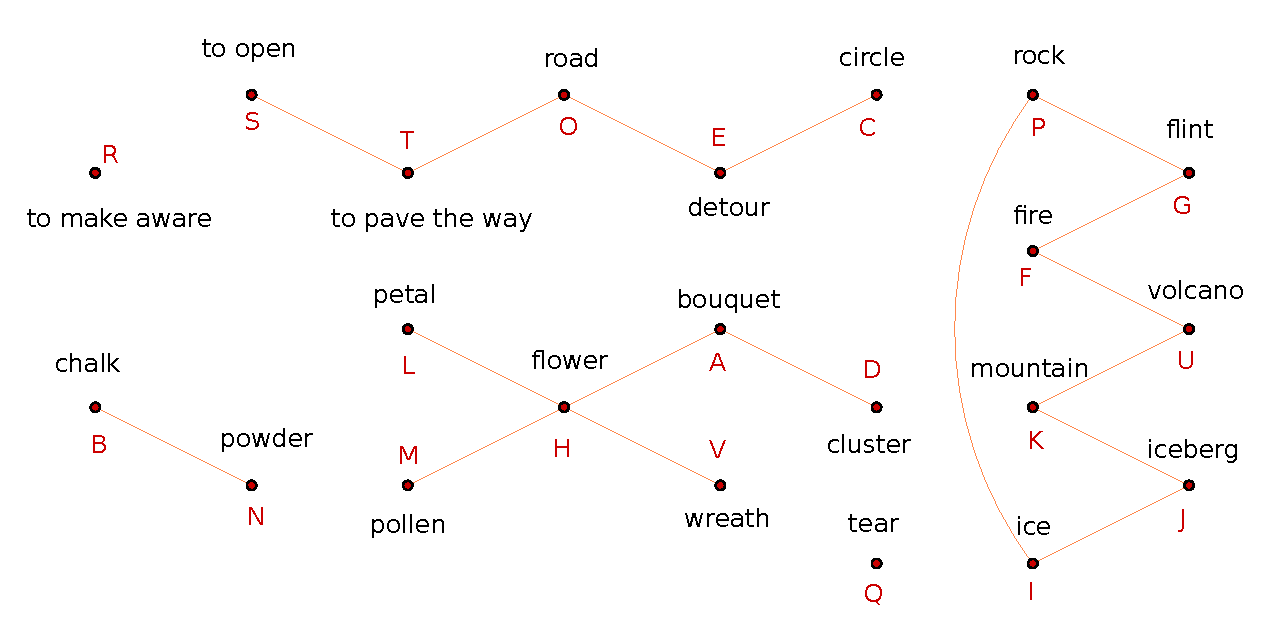
\includegraphics[width= 1\linewidth]{hc-2022-2-2-2-2.pdf}
	\caption{\small\textit{\color{toancuabi}Graph of English phrases}}
	\vspace*{-10pt}
\end{figure}  
Comparing the resulting graphs, only the $5-vertex$ subgraphs \textit{(phấn hoa, vòng hoa, cánh hoa, bó hoa, hoa)} and
\textit{(bouquet, petal, pollen, wreath, flower),} are \textit{isomorphic} (that is to say, they are the same graphs). Therefore, \textit{hoa}=\textit{flower}.
Observe that the relation between \textit{pollen} and \textit{power} implies that \textit{powder} is \textit{phấn}. The rest of the vertices can then be paired up
\textit{petal -- cánh hoa, bouquet -- bó hoa, pollen -- phấn hoa, wreath -- vòng hoa.}
Thus \textit{bó -- cluster} and \textit{chalk -- đá phấn}.
Similarly, the paths \textit{(băng -- núi băng -- núi -- núi lửa -- lửa -- đá lửa -- đá -- nước đá)} 
\textit{(ice -- iceberg -- mountain -- volcano -- fire -- flint -- rock)} are very much alike. In addition, the relation of \textit{đá -- đá phấn} is similar to \textit{rock - chalk}, and so both \textit{nước đá} and \textit{đá} mean \textit{ice}.
Similarly, the paths \textit{(vòng -- đường vòng -- đường -- mở đường -- mở)} 
\textit{(to open -- to pave the way -- road -- detour -- circle)} are very much alike.
\vskip 0.1cm
Following the same arguments, we can fill up the table below.
\end{multicols}
\begin{center}
	\renewcommand{\arraystretch}{1.2}
	\setlength{\tabcolsep}{8pt}
	\begin{tabular}{|c|l|l|c|l|}
		\hline
		$\#$ & Vietnamese & Literal meaning & Answer & English       \\ \hline
		$1 $ & băng       & ice             & I      & ice           \\ \hline
		$2 $ & bó         & cluster         & D      & cluster       \\ \hline
		$3 $ & bó hoa     & flower cluster  & A      & bouquet       \\ \hline
		$4 $ & cánh hoa   & flower wing     & L      & petal         \\ \hline
		$5 $ & đá         & rock            & P      & rock          \\ \hline
		$6 $ & đá lửa     & fire rock       & G      & flint         \\ \hline
		$7 $ & đá phấn    & powder rock     & B      & chalk         \\ \hline
		$8 $ & đường      & road            & O      & road          \\ \hline
		$9 $ & đường vòng & circle road     & E      & detour        \\ \hline
		$10$ & hoa        & flower          & H      & flower        \\ \hline
		$11$ & lửa        & fire            & F      & fire          \\ \hline
		$12$ & mở         & to open         & S      & to open       \\ \hline
		$13$ & mở đường   & to open a road  & T      & to pave a way \\ \hline
		$14$ & mở mắt     & to open eyes    & R      & to make aware \\ \hline
		$15$ & núi        & mountain        & K      & mountain      \\ \hline
		$16$ & núi băng   & ice mountain    & J      & iceberg       \\ \hline
		$17$ & núi lửa    & fire mountain   & U      & volcano       \\ \hline
		$18$ & nước đá    & rock water      & I      & ice           \\ \hline
		$19$ & nước mắt   & eye water       & Q      & tear          \\ \hline
		$20$ & phấn       & powder          & N      & powder        \\ \hline
		$21$ & phấn hoa   & flower powder   & M      & pollen        \\ \hline
		$22$ & vòng       & circle          & C      & circle        \\ \hline
		$23$ & vòng hoa   & flower circle   & V      & wreath        \\ \hline
	\end{tabular}
\end{center}